\documentclass[conference]{styles/acmsiggraph}

\usepackage{comment} % enables the use of multi-line comments (\ifx \fi)
\usepackage{lipsum} %This package just generates Lorem Ipsum filler text.
\usepackage{fullpage} % changes the margin
\usepackage{enumitem} % for customizing enumerate tags
\usepackage{amsmath,amsthm,amssymb}
\usepackage{listings}
\usepackage{graphicx}
\usepackage{etoolbox}   % for booleans and much more
\usepackage{verbatim}   % for the comment environment
\usepackage[dvipsnames]{xcolor}
\usepackage{fancyvrb}
\usepackage{hyperref}
\usepackage{menukeys}
\usepackage{titlesec}
\setlength{\parskip}{.8mm}
\usepackage{siunitx}
\usepackage{pdfpages}


\newtheorem{theorem}{Theorem}
\newtheorem{corollary}{Corollary}
\newtheorem{lemma}{Lemma}
\newtheorem{definition}{Definition}

\title{\huge Artificial Intelligence \\ \LARGE {Summary}}
\author{\Large Christian Schmidt \\ \Large Guido Battiston}
\pdfauthor{Christian Schmidt}

\hypersetup{
	colorlinks=true,
	urlcolor=[rgb]{0.97,0,0.30},
	anchorcolor={0.97,0,0.30},
	linkcolor=[rgb]{0.97,0,0.30},
	filecolor=[rgb]{0.97,0,0.30},
}

% redefine \VerbatimInput
\RecustomVerbatimCommand{\VerbatimInput}{VerbatimInput}%
{fontsize=\footnotesize,
 %
 frame=lines,  % top and bottom rule only
 framesep=2em, % separation between frame and text
 rulecolor=\color{Gray},
 %
 label=\fbox{\color{Black}\textbf{OUTPUT}},
 labelposition=topline,
 %
 commandchars=\|\(\), % escape character and argument delimiters for
                      % commands within the verbatim
 commentchar=*        % comment character
}

% convenient norm symbol
\newcommand{\norm}[1]{\left\lVert#1\right\rVert}
\renewcommand{\vec}[1]{\mathbf{#1}}

\usepackage{lastpage}
\usepackage{fancyhdr}
\pagestyle{fancy} 
\fancyfoot[CO,CE]{\thepage}

\titlespacing*{\section}{0pt}{5.5ex plus 1ex minus .2ex}{2ex}
\titlespacing*{\subsection}{0pt}{3ex}{2ex}

\setcounter{secnumdepth}{4}
\renewcommand\theparagraph{\thesubsubsection.\arabic{paragraph}}
\newcommand\subsubsubsection{\paragraph}

\setlength{\parskip}{0.5em}

% a macro for hiding answers
\newbool{hideanswers}
\setbool{hideanswers}{false}
\newenvironment{answer}{}{}
\ifbool{hideanswers}{\AtBeginEnvironment{answer}{\comment} %
\AtEndEnvironment{answer}{\endcomment}}{}

\newcommand{\points}[1]{\hfill \normalfont{(\textit{#1pts})}}
\newcommand{\pointsin}[1]{\normalfont{(\textit{#1pts})}}

\begin{document}
\maketitle

\tableofcontents
\newpage

\section{Intelligent Agents}

    \subsection{Ideal Rational Agent}
        Rational behavior is dependent on
        \begin{itemize}
            \item performance measures (goals)
            \item percept sequences
            \item knowledge of the environment
            \item possible actions
        \end{itemize}
        
        \textbf{Ideal Rational Agent}
        \textit{
            For each possible percept sequence, a rational agent should select an action that is expected to maximize its performance measure, given the evidence provided by the percept sequence and whatever built-in knowledge the agent has.
        }
        
        
    \subsection{Utility Function of Agent}
        \begin{itemize}
            \item The utility function is used \textbf{by the agent} to evaluate the desirability of a state of the world
            \item A utility function maps a state (or a sequence of states) onto an evaluation value (usually a real number)
            \item The agent can use the evaluation
                \begin{itemize}
                    \item to select an action (sequence)
                    \item to weigh the importance of competing goals
                \end{itemize}
        \end{itemize}

        $$Utility \times Percepts \times Knowledge \longrightarrow Action$$
        
        \begin{itemize}
            \item A selected action is \textbf{optimal} if it takes the agent to a state of maximum expected utility given available percepts and knowledge
            \item The agent is rational if it always chooses optimal actions
        \end{itemize}
        
        \includepdf[pages={30,31},nup=1x2]{ai0B_Intelligent_Agents.pdf}
        \includepdf[pages={35,36},nup=1x2]{ai0B_Intelligent_Agents.pdf}
        \includepdf[pages={39,41},nup=1x2]{ai0B_Intelligent_Agents.pdf}
        \includepdf[pages={45}]{ai0B_Intelligent_Agents.pdf}
        
        
\section{Systematic (Uninformed) Search}
    
    \subsection{Discrete State-Based Search Problems}
        \begin{itemize}
            \item \textbf{Discrete}\newline
                Finite number of states and actions
            \item \textbf{Single agent}\newline
                Do not consider action-based changes by other agents
            \item \textbf{Static}\newline
                World does not change while agent is deliberating
            \item \textbf{Observable}\newline
                Agent has access to relevant knowledge
            \item \textbf{Deterministic}\newline
                Each action has exactly one successor state $s \times a \longrightarrow s'$
        \end{itemize}
    
    \subsection{State Spaces}
        \subsubsubsection{Definition (State Space)}\ \\
            A \textbf{state space} is a 6-tuple $\Theta = (S,A,c,T,I,S^G)$ where:
            \begin{itemize}
                \item $S$ is a finite set of \textbf{states}.
                \item $A$ is a finite set of \textbf{actions}.
                \item $c : S \times A \implies \mathbb{R}^+_0$ is the \textbf{cost function}.
                \item $T \subseteq S \times A \times S$ is the \textbf{transition relation}.
                    We require that T is \textbf{deterministic}, i.e., for all $s \in S$ and $a \in A$, there is at most one state $s'$ such that $(s,a,s') \in T$.
                    If such $(s,a,s')$ exists, then $a$ is \textbf{applicable} to $s$.
                \item $I \in S$ is the \textbf{initial state}.
                \item $S^G \subseteq S$ is the set of \textbf{goal states}.
            \end{itemize}
            

        We say that $\Theta$ \textbf{has the transition} $(s,a,s')$ if $(s,a,s') \in T$.
        We also write $s \xrightarrow{a} s'$, or $s \rightarrow s'$ when not interested in $a$.
        We say that $\Theta$ has \textbf{unit costs} if, for all $a \in A$ and all $s \in S$, $c(s,a)=1$.
        

    \subsection{Terminology}
        \begin{itemize}
            \item $s'$ \textbf{successor} of $s$ if $s \rightarrow s'$; $s$ \textbf{predecessor} of $s'$ if $s \rightarrow s'$.
            \item $s'$ \textbf{reachable} from $s$ if there exists a sequence of transitions:
                $$s = s_0 \xrightarrow{a_1} s_1 \xrightarrow{a_2} ... \xrightarrow{a_{n-1}} s_{n-1} \xrightarrow{a_n} s_n = s'$$
                \begin{itemize}
                    \item $n=0$ possible; then $s=s'$.
                    \item $(a_1,...,a_n)$ is called \textbf{(action) path} from $s$ to $s'$.
                    \item $(s_0,...,s_n)$ is called \textbf{(state) path} from $s$ to $s'$.
                    \item The \textbf{cost} of that path is $\sum\limits_{i=1}^n c(s_{i-1},a_i)$.
                \end{itemize}
            \item $s'$ is \textbf{reachable} (without reference state) means reachable from $I$.
            \item $s$ is \textbf{solvable} if some $s' \in S^G$ is reachable from $s$; else $s$ is a \textbf{dead end}.
        \end{itemize}
    
    
    \subsection{(Optimal) State Space Solution}
        Let $\Theta = (S,A,c,T,I,S^G)$ be a state space, and let $s\in S$.
        \begin{itemize}
            \item A \textbf{solution} for $s$ is an action path $(a_1,...,a_n)$ from $s$ to some $s' \in S^G$.
            \item The solution is \textbf{optimal} if its cost is minimal among all solutions for $s$.
            \item A solution for $I$ is called a solution for $\Theta$ and denoted by $p$.
            \item The \textbf{set of all solutions} for $\Theta$ is denoted by $\mathbb{S}^{\Theta}$.
            \item If a solution exists, then $\Theta$ is \textbf{solvable}, otherwise \textbf{unsolvable}.
        \end{itemize}
        
        
        \includepdf[pages={12,13},nup=1x2]{ai01_Search_Systematic_Search.pdf}
        \includepdf[pages={14,15},nup=1x2]{ai01_Search_Systematic_Search.pdf}
        \includepdf[pages={16,17},nup=1x2]{ai01_Search_Systematic_Search.pdf}
        

    \subsection{Terminology to discuss Search Algorithms}
        \begin{itemize}
            \item \textbf{Search node n:}\newline
                Contains a $state$ reached by the search, plus information about how it was reached.
            \item \textbf{Path cost $g(n)$:}\newline
                The cost of the path reaching $n$.
            \item \textbf{Optimal cost $g^*$:}\newline
                The cost of an optimal solution path.
                For a state $s$, $g^*(s)$ is the cost of a cheapest path reaching $s$.
            \item \textbf{Node expansion:}\newline
                Generating all successors of a node, by applying all actions applicable to the node's state $s$.
                Afterwards, the state $s$ itself is also said to be expanded.
            \item \textbf{Search strategy:}\newline
                Method for deciding which node is expanded next.
            \item \textbf{Open list:}\newline
                Set of all $nodes$ that currently are candidates for expansion.
                Also called \textbf{frontier}.
            \item \textbf{Closed list:}\newline
                Set of all $states$ that were already expanded.
                Used only in \textbf{graph search}, not in \textbf{tree search} (up next).
                Also called \textbf{explored set}.
        \end{itemize}
    
    \subsection{Tree search vs. Graph Search}
        \begin{itemize}
            \item \textbf{Tree search}
                \begin{itemize}
                    \item We assume that the search space has tree structure
                    \item When performing tree search, we do not remember visited nodes, because one node can only be visited via exactly one path from the root of the tree (which represents the initial state)
                    \item However, with tree search on a graph we will not know whether we generate repeated states
                \end{itemize}
            \item \textbf{Graph Search}
                \begin{itemize}
                    \item Remember visited nodes (keep a closed list)
                    \item Use duplicate elimination: If a generated state is in the closed list, skip it, otherwise explore it
                \end{itemize}
        \end{itemize}
        
        
        \includepdf[pages={25,26},nup=1x2]{ai01_Search_Systematic_Search.pdf}
        \includepdf[pages={29,34},nup=1x2]{ai01_Search_Systematic_Search.pdf}
        \includepdf[pages={38,40},nup=1x2]{ai01_Search_Systematic_Search.pdf}
        \includepdf[pages={41,42},nup=1x2]{ai01_Search_Systematic_Search.pdf}
        \includepdf[pages={43,45},nup=1x2]{ai01_Search_Systematic_Search.pdf}
        \includepdf[pages={48,49},nup=1x2]{ai01_Search_Systematic_Search.pdf}
        
        
\section{Heuristic (Informed) Search}
    \subsection{Heuristic Functions $h$ and $h^*$}
        Let $\Pi$ be a problem with state space $\Theta$.
        A \textbf{heuristic function}, short \textbf{heuristic}, for $\Theta$ is a function $h: S \mapsto \mathbb{R}_0^+ \cup \{\infty\}$ so that, for every goal state $s$, we have $h(s) = 0$.\newline
        
        The \textbf{perfect heuristic} $h^*$ is the function assigning every $s \in S$ the cost of a cheapest path from $s$ to a goal state, or $\infty$ if no such path exists.
        
        \begin{itemize}
            \item $h(s) = \begin{cases} 0 & $if $s$ is a goal state$\\ >0 & $otherwise$ \end{cases}$
            \item $h^*(s) = \infty$ for dead-end states, from which the goal is unreachable
            \item $h^*(s)$ is also called the \textbf{goal distance} of $s$
            \item The value of $h$ depends only on the state $s$, not on the path that we followed so far to construct the partial solution (and the costs $g$ of this path)
        \end{itemize}
        
        
    \subsection{Desirable Properties of Heuristic Function $h(s)$}
        \begin{enumerate}
            \item Efficient to compute ($h(s) = 0$ as extreme case)
            \item Informative ($h(s) = h^*(s)$ as extreme case)
            \item $h(s) = \begin{cases} 0 & $if $s$ is a goal state$\\ >0 & $otherwise$ \end{cases}$
            \item $h$ is admissible
            \item $h(s_d) = \infty$ for dead-end states $s_d$
            \item $h$ is consistent\newline
        \end{enumerate}
        
        \begin{itemize}
            \item GOOD heuristics should satisfy a balanced compromise of properties (1) to (4) at least, better of all 6
            \item Properties (5) ensures effective dead-end recognition and (6) is a prerequisite for algorithms to guarantee minimal-cost (optimal) solution
        \end{itemize}
        
        
    \subsection{Admissiblity of $h(s)$}
        Let $\Pi$ be a problem with state space $\Theta$ and let $h$ be a heuristic function for $\Theta$.
        We say that $h$ is \textbf{admissible} if, for all $s \in S$, we have $h(s) \leq h^*(s)$.\newline
        
        The function $h^*(s)$ corresponds to the real cost of the optimal path from node $n$ to a goal state.\newline
        
        The function $h$ is an optimistic estimation of the costs that actually occur.
        It underestimates the real costs and provides the search algorithm with a lower bound on the goal distance.
        
        \includepdf[pages={9,10},nup=1x2]{ai02_Search_Heuristic_Search.pdf}
        \includepdf[pages={13,18},nup=1x2]{ai02_Search_Heuristic_Search.pdf}
        \includepdf[pages={34,37},nup=1x2]{ai02_Search_Heuristic_Search.pdf}
        \includepdf[pages={39,40},nup=1x2]{ai02_Search_Heuristic_Search.pdf}
        \includepdf[pages={41,42},nup=1x2]{ai02_Search_Heuristic_Search.pdf}
        
        
\section{Local and Stochastic Search}
    
    \subsection{Basic Idea of Local Search}
        \begin{itemize}
            \item Start somewhere in the search tree
            \item Use an evaluation function for each node
            \item Move towards better evaluated nodes
            \item Sometimes, move elsewhere
        \end{itemize}
    
    
    \subsection{Escape Techniques}
        \begin{itemize}
            \item \textbf{Tabu Search:}
                Add a memory to a local search algorithm to remember certain moves
                \begin{itemize}
                    \item keep a list of forbidden (visited) states
                    \item avoid moves that lead to previously explored regions of the search space\newline
                        (short term memory: do not reverse a previous move)
                    \item update this list while search progresses
                \end{itemize}
            \item \textbf{Random Restart:}
                Start over when no progress is made
                \begin{itemize}
                    \item do a random restart from a randomly generated initial state performing many hill climbing searches\newline
                        (theoretically complete, because it will eventually generate the goal state as an initial state)
                \end{itemize}
            \item \textbf{Random Walk:} 
                ''Inject noise'' = pick a worse or equal evaluated node with a certain probability
        \end{itemize}
    
    
    \subsection{Searching the Solution Space}
        \begin{itemize}
            \item In many applications, we do not care about the path to the solution
                \begin{itemize}
                    \item \textit{8 quenns:} the correct placement of queens on the board
                    \item \textit{cable tree wiring:} a robust and fast insertion order
                    \item \textit{vacuum world:} a plan that cleans all rooms
                \end{itemize}
            \item We can start with some randomly generated (partial) solution and try to improve it
                \begin{itemize}
                    \item take a solution node
                    \item generate its neighbors (if they have better evaluations)
                    \item do not keep information about the search path
                \end{itemize}
        \end{itemize}
    
    
    
\includepdf[pages={6,7},nup=1x2]{ai03_Search_Local_and_Stochastic_Search.pdf}
    
\includepdf[pages={18,20},nup=1x2]{ai03_Search_Local_and_Stochastic_Search.pdf}
    
    
    \subsection{Monte Carlo Algorithmus}
        Perform repeated random sampling to determine numerical estimations of unknown parameters
    
    \subsection{Monte Carlo Tree Search (MCTS)}
        \begin{itemize}
            \item Method for finding optimal decisions in a given domain by taking random samples in the decision space and building a search tree according to the results
                \begin{itemize}
                    \item statistical anytime algorithm for which more computing power generally leads to better performance
                    \item can be used with little or no domain knowledge
                \end{itemize}
            \item Since the 1990s, Monte Carlo ideas are applied to game playing and planning problems in AI
                \begin{itemize}
                    \item the method of choice for very large search spaces
                    \item $10^{120}$ and beyond
                    \item many variations and improvements exist
                \end{itemize}
        \end{itemize}


    \subsection{Summary}
        \begin{itemize}
            \item In very large search spaces heuristic search fails, we thus move to local and stochastic search methods and focus on anytime algorithms
            \item Stochastic and local search can converge to the optimal solution under very large resources (time, memory)
            \item UCT is the most popular stochastic search algorithm and has very successful applications in game playing
            \item Hillclimbing is a simple local search algorithm, which is very powerful when combined with random walks/moves and restarts
            \item A key to success for stochastic search is to find a good balance between exploration and exploitation
            \item Meta heuristic methods (such as genetic algorithms) do not guarantee optimality
                \begin{itemize}
                    \item as a result are not suitable for optimization
                    \item still very popular in practice they are good for finding a variety of well fitting solutions
                \end{itemize}
        \end{itemize}
    
    
    
\includepdf[pages={24,25},nup=1x2]{ai03_Search_Local_and_Stochastic_Search.pdf}
    
\includepdf[pages={26,27},nup=1x2]{ai03_Search_Local_and_Stochastic_Search.pdf}
    
\includepdf[pages={28,29},nup=1x2]{ai03_Search_Local_and_Stochastic_Search.pdf}
    
\includepdf[pages={30,31},nup=1x2]{ai03_Search_Local_and_Stochastic_Search.pdf}
    
    
    
    
\section{Propositional Logic}

    \subsection{Rationally Thinking Agent}
        Mathematical Logic provides us with a method to formalize the thinking “ of the agent
        \begin{itemize}
            \item Keep a knowledge base represented in logic
            \item Automate thinking by a logical calculus
        \end{itemize}
    
    
    \subsection{The Calculus of Propositional Logic}
        \begin{itemize}
            \item \textbf{Syntax:} What are structurally legal statements (formulas) in this logic?
            \item \textbf{Semantics:} What is the meaning of formulas?
            \item \textbf{Calculus:} Which rules and methods allow us to reason about formulas?
                \begin{itemize}
                    \item Find out if a formula/set of formulas is true or false?
                    \item Find out if a formula follows from another formula or set of formulas?
                \end{itemize}
        \end{itemize}
    
    
    \subsection{Syntax}
        Let $\Sigma$ be a set of boolean variables (atomic propositions). Then
        \begin{enumerate}
            \item $F(\bot)$ and $T(\top)$ are $\Sigma$-formulas (''false'', ''true'').
            \item Each $P \in \Sigma$ is a $\Sigma$-formula.
            \item If $\varphi$ is a $\Sigma$-formula, then so is $\lnot \varphi$ (''negation'').
            \item If $\varphi$ and $\psi$ are $\Sigma$-formulas, then so are
                \begin{enumerate}
                    \item $\varphi \land \psi$ (''conjunction'')
                    \item $\varphi \vee \psi$ (''disjunction'')
                    \item $\varphi \Rightarrow \psi$ (''implication'')
                    \item $\varphi \Leftrightarrow \psi$ (''equivalence'').
                \end{enumerate}
        \end{enumerate}
        Atoms and negated atoms are called \textbf{literals}.
    
    
    \subsection{Literal, Clause, and Sentence}
        \begin{itemize}
            \item \textbf{Literal}
                \begin{itemize}
                    \item atom
                    \item negation of an atom
                \end{itemize}
                Examples: $x_1, \lnot x_1$
            \item \textbf{Clause}
                \begin{itemize}
                    \item disjunction of literals
                \end{itemize}
                Examples: $(x_1 \vee x_2), (\lnot x_1 \vee x_2 \vee \lnot x_3)$
            \item \textbf{Sentence}
                \begin{itemize}
                    \item any atomic (literal) or complex proposition/sentence
                \end{itemize}
                Examples: $(x_1 \vee x_2) \Rightarrow (\lnot x_1 \vee x_2 \vee \lnot x_3), (x_1 \vee x_2) \land (\lnot x_1 \vee \lnot x_3)$
        \end{itemize}
    
    
    \subsection{Semantics}
        \begin{itemize}
            \item Defines the rules for determining the truth of a proposition/sentence with respect to an interpretation
            \item The interpretation assigns truth values to every proposition
        \end{itemize}
        
        Let $\Sigma$ be a set of propositions.
        An \textbf{interpretation} $I$ of $\Sigma$, also called a \textbf{truth assignment}, is a function
        $$I : \Sigma \rightarrow \{ 0,1 \}$$
    
    
    \subsection{Terminology}
        A knowledge Base (KB) is a set (conjunction) of formulas.\newline
        An interpretation is a model of KB if $I \vDash \varphi$ for all $\varphi \in KB$.\newline
        A formula $\varphi$ is:
            \begin{itemize}
                \item \textbf{satisfiable} iff there exists $I$ that satisfies $\varphi$
                \item \textbf{unsatisfiable} iff $\varphi$ is not satisfiable
                \item \textbf{falsifiable} iff there exists $I$ that doesn't satisfy $\varphi$
                \item \textbf{valid} iff $I \vDash \varphi$ holds for all $I$. We also call $\varphi$ a tautology.
            \end{itemize}
        
        Formulas $\varphi$ and $\psi$ are equivalent $(\varphi \equiv \psi)$ iff $M(\varphi) = M(\psi)$.
    
    
    \subsection{Important Equivalences}
        \begin{enumerate}
            \item $\lnot\lnot \varphi \equiv \varphi$
            \item $\lnot (\varphi \land \psi) \equiv (\lnot \varphi \vee \lnot \psi)$ (de Morgan)
            \item $\lnot (\varphi \vee \psi) \equiv (\lnot \varphi \land \lnot \psi)$ (de Morgan)
            \item $(\varphi \Leftrightarrow \psi) \equiv [(\varphi \Rightarrow \psi) \land (\psi \Rightarrow \varphi)]$
            \item $(\varphi \Rightarrow \psi) \equiv (\lnot \varphi \vee \psi)$
            \item $\varphi \land (\psi \vee \chi) \equiv (\varphi \land \psi) \vee (\varphi \land \chi)$ (distributivity)
            \item $\varphi \vee (\psi \land \chi) \equiv (\varphi \vee \psi) \land (\varphi \vee \chi)$ (distributivity)
            \item $\varphi \land \lnot \varphi \equiv F$
            \item $\varphi \vee \lnot \varphi \equiv T$
        \end{enumerate}
    
    
    \subsection{Normal Forms}
        \begin{itemize}
            \item A formula is in \textbf{conjunctive normal form (CNF)} if it consists of a conjunction of disjunctions of literals:
             $$\bigwedge\limits_{i=1}^n \Biggl(\bigvee\limits_{j=1}^{m_i} l_{i,j} \Biggr)$$
             \item A formula is in \textbf{disjunctive normal form (DNF)} if it consists of a conjunction of disjunctions of literals:
             $$\bigvee\limits_{i=1}^n \Biggl(\bigwedge\limits_{j=1}^{m_i} l_{i,j} \Biggr)$$
        \end{itemize}
    
    
    \subsection{Calculus}
        How can we find out $KB \vDash \varphi$?
        \begin{enumerate}
            \item By the truth table method, but $n$ boolean variables require to consider $2^n$ truth value combinations
            \item Using the contradiction theorem, we can try to derive with the help of inference rules (a „calculus“) that
                $$KB \cup \{ \lnot \varphi \} \vDash \bot$$
        \end{enumerate}
    
    
    \subsection{Soundness and Completeness of a Calculus}
        A formula $\varphi$ can be derived from a knowledge base $KB$ using a calculus $\mathcal{R}$
            $$KB \vdash_{\mathcal{R}} \varphi$$
        iff there is a deriviation using rules from $\mathcal{R}$ ending in $\varphi$.\newline
        
        \textbf{Soundness:} $\mathcal{R}$ is sound iff all derivable formulas follow logically:
            $$if \  KB \vdash_{\mathcal{R}} \varphi, \  then \  KB \vDash \varphi.$$
        
        \textbf{Completeness:} $\mathcal{R}$ is complete if all formulas that follow logically are derivable:
            $$if \  KB \vDash \varphi, \  then \  KB \vdash_{\mathcal{R}} \varphi.$$
        
        If $\mathcal{R}$ is \textbf{sound} and \textbf{complete}:
            $$KB \vDash \varphi \Leftrightarrow KB \vdash_{\mathcal{R}} \varphi.$$
    


    \includepdf[pages={16,19},nup=1x2]{ai04_Propositional_Logic.pdf}
    \includepdf[pages={20,21},nup=1x2]{ai04_Propositional_Logic.pdf}
    \includepdf[pages={25,27},nup=1x2]{ai04_Propositional_Logic.pdf}
    \includepdf[pages={31,32},nup=1x2]{ai04_Propositional_Logic.pdf}
    \includepdf[pages={33,34},nup=1x2]{ai04_Propositional_Logic.pdf}
    
    
    \subsection{SAT Checking}
        \begin{itemize}
            \item Is an (arbitrary) formula $\varphi$ satisfiable?
                \begin{itemize}
                    \item Yes, if we can construct a model of $\varphi$
                    \item Find a truth assignment (a satisfying interpretation ) for the boolean variables in $\varphi$ making the formula true
                    \item If no model exists, return unsatisfiable
                \end{itemize}
            \item If $KB \cup \{ \lnot \varphi \}$ is unsatisfiable, then $KB \vDash \varphi$ (by the contradiction theorem)
                \begin{itemize}
                    \item SAT checking can be used like a calculus
                \end{itemize}
        \end{itemize}
    
    
    \subsection{Characterization of Clauses Disjunction of Literals)}
        \begin{itemize}
            \item \textbf{Unsatisfied} if all its literals are assigned value 0 (false)
            \item \textbf{Satisfied} if at least one of its literals is assigned value 1 (true)
            \item \textbf{Unit} if all literals but one are assigned value 0, and the remaining literal is unassigned
                \begin{itemize}
                    \item This remaining literal must be assigned 1
                \end{itemize}
            \item \textbf{Unresolved} if it is neither unsatisfied, nor satisfied, nor unit
        \end{itemize}
    
    
    \includepdf[pages={46,47},nup=1x2]{ai04_Propositional_Logic.pdf}
    \includepdf[pages={48,49},nup=1x2]{ai04_Propositional_Logic.pdf}
    \includepdf[pages={50,51},nup=1x2]{ai04_Propositional_Logic.pdf}
    
    \includepdf[pages={56,57},nup=1x2]{ai04_Propositional_Logic.pdf}
    \includepdf[pages={58,59},nup=1x2]{ai04_Propositional_Logic.pdf}
    \includepdf[pages={60,64},nup=1x2]{ai04_Propositional_Logic.pdf}
    

    
    
\section{Predicate Logic Reasoning, Part I: Basics}

    \subsection{The Alphabet of PL1}
        \begin{itemize}
            \item General symbols:
                \begin{itemize}
                    \item \textbf{Variables:} $x,x_1,x_2,...,x',x'',...,y,...,z,...$
                    \item \textbf{Truth/Falseness:} $\top,\bot$. (As in propositional logic)
                    \item \textbf{Operators:} $\lnot,\vee,\wedge,\rightarrow,\leftrightarrow$. (As in propositional logic)
                    \item \textbf{Quantifiers:} $\forall,\exists$.\newline
                        $\rightarrow$ Precedence: $\lnot \  > \  \forall$, $\exists \  > \  ... \ $ (we'll be using brackets).
                \end{itemize}
            \item Application-specific symbols:
                \begin{itemize}
                    \item \textbf{Constant symbols} (''object'', e.g., $BlockA,BlockB,a,b,c,...$)
                    \item \textbf{Predicat symbols, arity} $\geq 1$ (e.g., $Block(.),Above(.,.)$)
                    \item \textbf{Function symbols, arity} $\geq 1$ (e.g., $WeightOf(.),Succ(.)$)
                \end{itemize}
        \end{itemize}
    
    
    \subsection{Definition (Signature)}
        A signature $\Sigma$ in predicate logic is a finite set of constant symbols, predicate symbols, and function symbols.\newline
        \textbf{$\rightarrow$ In mathematics, $\Sigma$ can be infinite; not considered here.}
    
    
    \subsection{Syntax of PL1}
        \textbf{$\rightarrow$ Terms represent objects:}
        \subsubsection{Definition (Term)}
            Let $\Sigma$ be a signature. Then:
            \begin{enumerate}
                \item Every variable and every constant symbol is a \textbf{$\Sigma$-term}.
                \item If $t_1,t_2,...,t_n$ are $\Sigma$-terms and $f \in \Sigma$ is an $n$-ary function symbol, then $f(t_1,t_2,...,t_n)$ also is a $\Sigma$-term.
            \end{enumerate}
            Terms without variables are \textbf{ground terms}.\newline
        $\rightarrow$ For simplicity, we usually don't write the ''$\Sigma$-''.\newline
        
        \textbf{$\rightarrow$ Atoms represent atomic statements about objects:}
        \subsubsection{Definition (Atom)}
            Let $\Sigma$ be a signature. Then:
            \begin{enumerate}
                \item $\top$ and $\bot$ are $\Sigma$-\textbf{atoms}.
                \item If $t_1,t_2,...,t_n$ are terms and $P \in \Sigma$ is an $n$-ary predicate symbol, then $P(t_1,t_2,...,t_n)$ is a $\Sigma$-atom.
            \end{enumerate}
            Atoms without variables are \textbf{ground atoms}.
        
        \textbf{$\rightarrow$ Formulas represent complex statements about objects:}
        \subsubsection{Definition (Formula)}
            Let $\Sigma$ be a signature. Then:
            \begin{enumerate}
                \item[1.] Each $\Sigma$-atom is a \textbf{$\Sigma$-formula}.
                \item[2.] If $\varphi$ is a $\Sigma$-formula, then so is $\lnot \varphi$.
            \end{enumerate}
            The formulas that can be constructed by rules 1. and 2. are \textbf{literals}.\newline
            If $\varphi$ and $\psi$ are $\Sigma$-formulas, then so are:
            \begin{enumerate}
                \item[3.] $\varphi \wedge \psi, \varphi \vee \psi, \varphi \rightarrow \psi$, and $\varphi \leftrightarrow \psi$.
            \end{enumerate}
            If $\varphi$ is a $\Sigma$-formula and $x$ is a variable, then
            \begin{enumerate}
                \item[4.] $\forall x \varphi$ is a $\Sigma$-formula (''Universal Quantification'').
                \item[5.] $\exists x \varphi$ is a $\Sigma$-formula (''Existential Quantification'').
            \end{enumerate}
        
    \subsection{The Meaning of PL1 Formulas}
        \subsubsection{Example:}
            $$\forall x [Block(x) \rightarrow Red(x)], Block(A)$$
            $\rightarrow$ For all objects $x$, if $x$ is a block, then $x$ is red. $A$ is a block.
        
        \subsubsection{More generally: (Intuition)}
            \begin{itemize}
                \item Terms represent objects.
                \item Predicates represent relations on the universe.
                \item Universally-quantified variables: ''for all objects in the universe''.
                \item Existentially-quantified variables: ''at least one object in the universe''.
            \end{itemize}
            $\rightarrow$ Similar to propositional logic, we define interpretations, models, satisfiability, validity, ...
    
    \subsection{Semantics of PL1: Interpretations}
        \subsubsection{Definition (Interpretation)}
            Let $\Sigma$ be a signature.
            A \textbf{$\Sigma$-interpretation} is a pair $(U,I)$ where $U$, the \textbf{universe}, is an arbitrary non-empty set, and $I$ is a function, notated as superscript, so that
            \begin{enumerate}
                \item $I$ maps constant symbols to elements of $U$: $c^I \in U$
                \item $I$ maps $n$-ary predicate symbols to $n$-ary relations over $U$: $P^I \subseteq U^n$
                \item $I$ maps $n$-ary function symbols to $n$-ary functions over $U$: $f^I \in [U^n \mapsto U]$
            \end{enumerate}
        \textbf{$\rightarrow$ We will often refer to $I$ as the interpretation, omitting $U$. Note that $U$ may be infinite.}
        
        \subsubsection{Definition (Ground Term Interpretation)}
            The interpretation of a ground term under $I$ is $(f(t_1,...,t_n))^I = f^I (t^I_1,...,t^I_n)$.
        
        \subsubsection{Definition (Ground Atom Satisfaction)}
            Let $\Sigma$ be a signature and $I$ a $\Sigma$-interpretation.\newline
            We say that $I$ \textbf{satisfies} a ground atom $P(t_1,...,t_n)$, written $I \vDash P(t_1,...,t_n)$, iff $(t^I_1,...,t^I_n) \in P^I$.\newline
            We also call $I$ a \textbf{model} of $P(t_1,...,t_n)$.
        
    
    \subsection{Semantics of PL1: Variable Assignments}
        \subsubsection{Variable Assignment}
            Let $\Sigma$ be a signature and $(U,I)$ a $\Sigma$-interpretation.\newline
            Let $X$ be the set of all variables.\newline
            A \textbf{variable assignment $\alpha$} is a function $\alpha : X \mapsto U$.
        
        \subsubsection{Definition (Term Interpretation)}
            The interpretation of a term under $I$ and $\alpha$ is:
            \begin{enumerate}
                \item $x^{I,\alpha} = \alpha(x)$
                \item $c^{I,\alpha} = c^I$
                \item $(f(t_1,...,t_n))^{I,\alpha} = f^I(t^{I,\alpha}_1,...,t^{I,\alpha}_n)$
            \end{enumerate}
        
        \subsubsection{Definition (Atom Satisfaction)}
            Let $\Sigma$ be a signature, $I$ a $\Sigma$-interpretation, and $\alpha$ a variable assignment.\newline
            We say that $I$ and $\alpha$ \textbf{satisfy} an atom $P(t_1,...,t_n)$, written $I$, $\alpha \vDash P(t_1,...,t_n)$, iff $(t^{I,\alpha}_1,...,t^{I,\alpha}_n) \in P^I$.\newline
            We also call $I$ and $\alpha$ a \textbf{model} of $P(t_1,...,t_n)$.
    
    
    \subsection{Semantics of PL1: Formula Satisfaction}
        \subsubsection{Notation}
            In $\alpha \frac{x}{o}$ we overwrite $x$ with $o$ in $\alpha:$ for $\alpha = \{(x \mapsto o_1),(y \mapsto o_2),,...\}$, $\alpha \frac{x}{o} = \{(x \mapsto o),(y \mapsto o_2),,...\}$.
        
        \subsubsection{Definition (Formula Satisfaction)}
            Let $\Sigma$ be a signature, $I$ a $\Sigma$-interpretation, and $\alpha$ a variable assignment. We set:
                \begin{itemize}
                    \item $I, \alpha \vDash \top$ and $I, \alpha \nvDash \bot$
                    \item $I, \alpha \vDash \lnot \varphi$ iff $I, \alpha \nvDash \varphi$
                    \item $I, \alpha \vDash \varphi \wedge \psi$ iff $I, \alpha \vDash \varphi$ and $I, \alpha \vDash \psi$
                    \item $I, \alpha \vDash \varphi \vee \psi$ iff $I, \alpha \vDash \varphi$ or $I, \alpha \vDash \psi$
                    \item $I, \alpha \vDash \varphi \rightarrow \psi$ iff if $I, \alpha \vDash \varphi$, then $I, \alpha \vDash \psi$
                    \item $I, \alpha \vDash \varphi \leftrightarrow \psi$ iff if $I, \alpha \vDash \varphi$ if and only if $I, \alpha \vDash \psi$
                    \item $I, \alpha \vDash \forall x \varphi$ iff for all $o \in U$ we have $I, \alpha \frac{x}{o} \vDash \varphi$
                    \item $I, \alpha \vDash \exists x \varphi$ iff there exists $o \in U$ so that $I, \alpha \frac{x}{o} \vDash \varphi$
                \end{itemize}
            If $I, \alpha \vDash \varphi$, we say that $I$ and $\alpha$ \textbf{satisfy} $\varphi$ (are a \textbf{model} of $\varphi$).
        
    \subsection{PL1 Satisfiability}
        \subsubsection{Satisfiability}
            A PL1 formula $\varphi$ is:
            \begin{itemize}
                \item \textbf{satisfiable} if there exist $I, \alpha$ that satisfy $\varphi$.
                \item \textbf{unsatisfiable} if $\varphi$ is not satisfiable.
                \item \textbf{falsifiable} if there exist $I, \alpha$ that do not satisfy $\varphi$.
                \item \textbf{valid} if $I, \alpha \vDash \varphi$ holds for all $I$ and $\alpha$.
                    We also call $\varphi$ a \textbf{tautology}.
            \end{itemize}
            
        \subsubsection{Entailment and Equivalence}
            $\varphi$ \textbf{entails} $\psi$, $\varphi \vDash \psi$, if every model of $\varphi$ is a model of $\psi$.\newline
            $\varphi$ and $\psi$ are \textbf{equivalent}, $\varphi \equiv \psi$, if $\varphi \vDash \psi$ and $\psi \vDash \varphi$.
            
            
    \subsection{Free and Bound Variables}
        \subsubsection{Definition (Free Variables)}
            By $vars(e)$, where $e$ is either a term or a formula, we denote the set of variables occuring in $e$. We set:
            \begin{itemize}
                \item $free(P(t_1,...,t_n)) := vars(t_1) \cup ... \cup vars(t_n)$
                \item $free(\lnot \varphi) := free(\varphi)$
                \item $free(\varphi \ast \psi) := free(\varphi) \cup free(\psi)$ for $\ast \in \{\wedge,\vee,\rightarrow,\leftrightarrow\}$
                \item $free(\forall x \varphi) := free(\varphi) \backslash \{x\}$
                \item $free(\exists x \varphi) := free(\varphi) \backslash \{x\}$
            \end{itemize}
            $free(\varphi)$ are the \textbf{free variables} of $\varphi$. $\varphi$ is \textbf{closed} if $free(\varphi) = \emptyset$.\newline
            $\rightarrow$ Knowledge Base (aka \textbf{logical theory}) = set of closed formulas. From now on, we asume that $\varphi$ is closed.\newline
            $\rightarrow$ We can ignore $\alpha$, and will write $I \vDash \varphi$ instead of $I, \alpha \vDash \varphi$.
\newpage            
            
        \subsubsection{Why normal forms?}
            \begin{itemize}
                \item \textbf{Convenient:} full syntax when \textit{describing the problem} at hand.
                \item \textbf{Not convenient:} full syntax when \textit{solving the problem}.
            \end{itemize}
        
        \subsubsection{''Solving the problem''? Decide satisfiability!}
            $\rightarrow$ Tackles deduction as well as other applications. (Same as in propositional logic)

        \subsubsection{Prenex-, Skolem- and Clausal normal form}
            \begin{itemize}
                \item \textbf{Prenex normal form:} Move all quantifiers up front.
                \item \textbf{Skolem normal form:} Prenex, + remove all existential quantifiers while preserving satisfiability.
                \item \textbf{Clausal normal form:} Skolem, + CNF transformation while preserving satisfiability.
            \end{itemize}
        
    \subsection{Summary}
        \begin{itemize}
            \item \textbf{First-order predicate logic (PL1)} allows \textbf{universal} and \textbf{existential} quantification over objects.
            \item A PL1 \textbf{interpretation} consists of a \textbf{universe $U$} and a function $I$ mapping \textbf{constant symbols/predicate symbols/function symbols} to elements/relations/functions on $U$.
            \item In \textbf{prenex normal form}, all quantifiers are up front. In \textbf{Skolem normal form}, additionally there are no existential quantifiers. In \textbf{clausal normal form}, additionally the formula is in CNF.
            \item Any PL1 formula can eficiently be brought into a satisfiability-equivalent clausal normal form.
        \end{itemize}
    
    
    \includepdf[pages={29,30},nup=1x2]{ai05_POST-HANDOUT_Predicate_Logic_I.pdf}
    \includepdf[pages={31,32},nup=1x2]{ai05_POST-HANDOUT_Predicate_Logic_I.pdf}
    \includepdf[pages={33,35},nup=1x2]{ai05_POST-HANDOUT_Predicate_Logic_I.pdf}
    \includepdf[pages={36,37},nup=1x2]{ai05_POST-HANDOUT_Predicate_Logic_I.pdf}
    
    
    
    
\section{Predicate Logic Reasoning, Part II: Reasoning}
    \subsection{Herbrand: The Infinite Case}
        $\rightarrow$ \textbf{Recall:} Without function symbols, the Herbrand expansion is finite, and PL1 reasoning is equivalent to propositional reasoning.
        
        \subsubsection{Theorem (Compactness of Propositional Logic)}
            Any set $\theta$ of propositional logic formulas is unsatisfiable if and only if at least one finite subset of $\theta$ is unsatisfiable. (Proof omitted.)
        
        \subsubsection{Method:}
            Enumerate all finite subsets $\theta_1$ of the Herbrand expansion $HE(\theta^*)$, and test propositional satisfiability of $\theta_1$.
            $\theta$ is unsatisfiable if and only if one of the $\theta_1$ is.
        
        $\rightarrow$ If the Herbrand expansion is infinite, to show unsatisfiability (= to prove that some property does indeed follow from the KB), we must somehow choose a ''relevant'' finite subset thereof.
        
        
    \subsection{Herbrand, Infinite Case: What If $\theta$ is Satisfiable?}
        \subsubsection{Theorem (A)}
            The set of unsatisfiable PL1 formulas is recursively enumerable.
        
        \subsubsection{Proof Theorem (A)}
            Enumerate all PL1 formulas $\varphi$. 
            Incrementally for all of these in parallel, enumerate all finite subsets $\theta_1$ of the Herbrand expansion $HE(\varphi^*)$.
            Test propositional satisfiability of each $\theta_1$. 
            By compactness of propositional logic, if $HE(\varphi^*)$ is unsatisfiable then one of the $\theta_1$ is.
        
        \subsubsection{Theorem (B)}
            It is undecidable whether a PL1 formula is satisfiable. (Proof omitted.)
        
        \subsubsection{Corollary}
            The set of satisfiable PL1 formulas is not recursively enumerable. 
            (Proof: Else, with Theorem (A), PL1 satisfiability would be decidable, in contradiction to Theorem (B).)
        
        $\rightarrow$ If a PL1 formula is unsatisfiable, then we can confirm this. 
            Otherwise, we might end up in an infinite loop.
    
    
    \includepdf[pages={7,8},nup=1x2]{ai06_POST-HANDOUT_Predicate_Logic_I_I.pdf}
    \includepdf[pages={14,15},nup=1x2]{ai06_POST-HANDOUT_Predicate_Logic_I_I.pdf}
    \includepdf[pages={16,17},nup=1x2]{ai06_POST-HANDOUT_Predicate_Logic_I_I.pdf}
    \includepdf[pages={18,19},nup=1x2]{ai06_POST-HANDOUT_Predicate_Logic_I_I.pdf}
    
    
    \subsection{Unification}
        \subsubsection{Definition (Unifier)}
            We say that a substitution $s$ is a \textbf{unifier} for a set of atoms $\{P_1,...,P_k\}$ if $P_is = P_js$ for all $i,j$.\newline
            \textbf{Notation:} We'll usually write $\{P_i\}$ for $\{P_1,...,P_k\}$.\newline
            \textbf{Example:} $\{P(x,f(y,z),b),P(x,f(b,w),b)\}$\newline
                $\rightarrow$ $s = \{\frac{y}{b},\frac{z}{w},\frac{x}{h(a,b)}\}$? Yes. But not ''the best'' one.\newline
                $\rightarrow$ $s = \{\frac{y}{b},\frac{z}{w}\}$? Yes. This is a \textbf{most general unifier (MGU):}
            
        \subsubsection{Definition (MGU)}
            We say that a unifier \textbf{g} of $\{P_i\}$ is an \textbf{MGU} if, for any unifier $s$ of $\{P_i\}$, there exists a substitution $s'$ s.t. $\{P_i\}s = \{P_i\}gs'$.
        
        $\rightarrow$ If any unifier exists, then an idempotent MGU exists.\newline
        $\rightarrow$ We'll next introduce an algorithm that finds it.
        
    \subsection{Disagreement Set}
        \subsubsection{Definition (Disagreement Set)}
            The \textbf{disagreement set $D(\{t_i\})$} of a set of terms $\{t_i\}$ is the leftmost and outermost set of sub-terms where some of the $t_i$ disagree.$^1$\newline
            The \textbf{disagreement set $D(\{P_i\})$} of a set of atoms $\{P_i\}$ is the disagreement set $D(\{t_i\})$ where $\{t_i\}$ is the term set at the leftmost argument for which some of the $P_i$ disagree.
        
        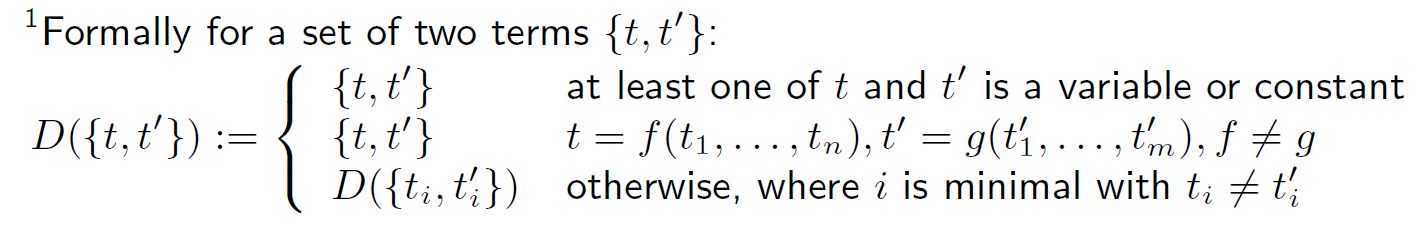
\includegraphics[width=0.85\textwidth]{imgs/DisagreementSet.png}
        
        \subsubsection{Examples}
            \begin{itemize}
                \item $\{P(x,c,f(y)),P(x,z,z)\}: \{c,z\}$
                \item $\{P(x,a,f(y)),P(y,a,f(y))\}: \{x,y\}$
                \item $\{P(v,f(z),g(w)),P(v,f(z),g(f(z)))\}: \{w,f(z)\}$
                \item $\{P(v,f(z),g(w)),P(v,f(z),g(f(z))),P(v,f(z),f(x))\}: \{g(w),g(f(z)),f(x)\}$
            \end{itemize}

\newpage

    \subsection{Summary}
        \begin{itemize}
            \item The \textbf{Herbrand universe} is the set of all ground terms that can be built from the symbols used in a set $\theta$ of PL1 formulas. 
                The (propositional-logic) \textbf{Herbrand expansion} instantiates the formulas with these terms, and is satisfiable iff $\theta$ is.
            \item For unsatisfiable $\theta$, we can always find an unsatisfiable finite subset of the Herbrand expansion.
            \item \textbf{PL1 resolution} reasons directly about PL1 formulas (in clausal normal form).
                It relies on \textbf{unification} to compare PL1 terms.
            \item \textbf{Binary PL1 resolution} is like propositional resolution with unification. 
                It is not refutation-complete.
            \item To obtain a complete PL1 resolution calculus, we can either allow to unify sets of resolution literals (\textbf{full PL1 resolution}), or to unify literals within clauses (\textbf{factoring}).
            \item The set of satisfiable PL1 formulas is not recursively enumerable. 
                Thus, neither the reduction to propositional logic, nor PL1 resolution, guarantee to terminate in finite time.
        \end{itemize}

        
    \includepdf[pages={23,24},nup=1x2]{ai06_POST-HANDOUT_Predicate_Logic_I_I.pdf}
    \includepdf[pages={26,27},nup=1x2]{ai06_POST-HANDOUT_Predicate_Logic_I_I.pdf}
    \includepdf[pages={29,30},nup=1x2]{ai06_POST-HANDOUT_Predicate_Logic_I_I.pdf}
    
    \includepdf[pages={32,33},nup=1x2]{ai06_POST-HANDOUT_Predicate_Logic_I_I.pdf}
    \includepdf[pages={34,35},nup=1x2]{ai06_POST-HANDOUT_Predicate_Logic_I_I.pdf}
    \includepdf[pages={36,37},nup=1x2]{ai06_POST-HANDOUT_Predicate_Logic_I_I.pdf}



\section{Adversarial Search}
    \subsection{These Games: Restrictions}
        \begin{itemize}
            \item The game state is \textbf{fully observable}.
            \item The outcome of each move is \textbf{deterministic}.
            \item Game states \textbf{discrete, finite} number of possible moves and game states.
            \item There are \textbf{no infinite runs} of the game: a \textbf{terminal state} is always reached after a finite number of steps.
            \item \textbf{Two-player zero-sum} game: two players, terminal states have utility with utility(player1) = -utility(player2).
            \item Our formulation (equivalent): single \textbf{utility function $u$}, players $Max$ vs. $Min$ trying to \textbf{maximize vs. minimize $u$}.
            \item \textbf{Turn-taking:} Players move alternatingly. Max begins.
        \end{itemize}
    
    \subsection{Formalization}
        \subsubsection{Definition (Game State Space)}
            A \textbf{game state space} is a 6-tuple $\Theta = (S,A,T,I,S^T,u)$ where:
                \begin{itemize}
                    \item $S,A,T,I$: States, actions, deterministic transition relation, initial state. 
                        As in classical search problems, except:
                            \begin{itemize}
                                \item $S$ is the disjoint union of $S^{Max},S^{Min}$, and $S^T$.
                                \item $A$ is the disjoint union of $A^{Max}$ and $A^{Min}$.
                                \item For $a \in A^{Max}$, if $s \xrightarrow{a} s'$ then $s \in S^{Max}$ and $s' \in S^{Min} \cup S^T$.
                                \item For $a \in A^{Min}$, if $s \xrightarrow{a} s'$ then $s \in S^{Min}$ and $s' \in S^{Max} \cup S^T$.
                            \end{itemize}
                        \item $S^T$ is the set of \textbf{terminal states}.
                        \item $u : S^T \mapsto \mathbb{R}$ is the \textbf{utility function}.
                \end{itemize}
        
        \subsubsection{Commonly used terminology:}
            \begin{itemize}
                \item state = \textbf{position}
                \item terminal state = \textbf{end state}
                \item action = \textbf{move}
            \end{itemize}
            (A round of the game - one move Max, one move Min - is often referred to as a ''move'', and individual actions as ''half-moves''. We do NOT do that here.)
        
    
    \subsection{Why Games are Hard to Solve}
        \subsubsection{Definition (Policy)}
            Let $\Theta$ be a game state space, and let $X \in \{Max,Min\}$.
            A \textbf{policy} for $X$ is a function $p^X : S^X \mapsto A^X$ so that $a$ is applicable to $s$ whenever $p^X(s)=a$.
            \begin{itemize}
                \item We don't know how the opponent will react, and need to \textbf{prepare for all possibilities}.
                \item A policy is \textbf{optimal} if it yields the best possible utility for $X$ assuming perfect opponent play (not formalized here).
                \item In (almost) all games, computing a policy is infeasible. Instead, compute the next move ''on demand'', given the current game state.
            \end{itemize}
        
    \subsection{Agenda for This Chapter}
        \begin{itemize}
            \item \textbf{Minimax Search:} How to compute an optimal policy?\newline
                $\rightarrow$ \textit{Minimax is the canonical (and easiest to understand) algorithm for solving games, i.e., computing an optimal policy.}
            \item \textbf{Alpha-Beta Search:} How to prune unnecessary parts of the tree?\newline
                $\rightarrow$ \textit{An essential improvement over Minimax.}
            \item \textbf{Evaluation Functions:} How to evaluate a game position?\newline
                $\rightarrow$ \textit{Heuristic functions for games, and how to obtain them.}
            \item \textbf{AlphaGo/Zero:} How does it work?\newline
                $\rightarrow$ \textit{Overview of the AlphaGo/Zero systems architecture.}
        \end{itemize}
    
    \subsection{Minimax}
        \textbf{We max, we min, we max, we min...}
        \begin{enumerate}
            \item Depth-first search in game tree, with Max in the root.
            \item Apply utility function to terminal positions.
            \item Bottom-up for each inner node $n$ in the tree, compute the utility $u(n)$ of $n$ as follows:
                \begin{itemize}
                    \item If it's Max's turn: Set $u(n)$ to the maximum of the utilities of $n$'s successor nodes.
                    \item If it's Min's turn: Set $u(n)$ to the minimum of the utilities of $n$'s successor nodes.
                \end{itemize}
            \item Selecting a move for Max at the root: Choose one move that leads to a successor node with maximal utility.
        \end{enumerate}
    
    \subsection{Minimax, Pro and Contra}
        \begin{itemize}
            \item \textbf{Pro:}
                \begin{itemize}
                    \item Returns an optimal action, assuming perfect opponent play.
                    \item Extremely simple.
                \end{itemize}
            \item \textbf{Contra:}
                \begin{itemize}
                    \item \textit{Completely infeasible (search tree way too large).}
                \end{itemize}
            \item \textbf{Remedies:}
                \begin{itemize}
                    \item Limit search depth, apply \textit{evaluation function} at cut-off states.
                    \item Sparse search (MCTS) instead of exhaustive search.
                    \item \textit{Alpha-beta} pruning reduces search yet preserves optimality.
                \end{itemize}
        \end{itemize}
    
    
    \includepdf[pages={18,19},nup=1x2]{ai07_POST-HANDOUT_Adversarial_Search.pdf}
    \includepdf[pages={27,29},nup=1x2]{ai07_POST-HANDOUT_Adversarial_Search.pdf}
    
    \includepdf[pages={33,34},nup=1x2]{ai07_POST-HANDOUT_Adversarial_Search.pdf}
    \includepdf[pages={38,39},nup=1x2]{ai07_POST-HANDOUT_Adversarial_Search.pdf}
    \includepdf[pages={40,48},nup=1x2]{ai07_POST-HANDOUT_Adversarial_Search.pdf}
    \includepdf[pages={52,53},nup=1x2]{ai07_POST-HANDOUT_Adversarial_Search.pdf}
    
    
    \subsection{Evaluation Functions}
        \subsubsection{Definition}
            Given a game with states $S$, a \textbf{(heuristic) evaluation function} is a function $h : S \mapsto \mathbb{R}$.
                \begin{itemize}
                    \item \textbf{$h$ estimates the expected utility of $s$.}
                        (In particular, we can use $h := u$ on terminal states)
                    \item In Minimax: Impose depth limit, use $h$ at (non-terminal) cut-off states.
                    \item In MCTS: Use $h$ as part of the state-value estimates. 
                        (e.g. AlphaGo: leaf state value estimate is linear combination of $h$ and rollouts)
                \end{itemize}
        
    \subsection{Linear Feature-Based Evaluation Functions}
        \subsubsection{Functions taking the form:}
            $$h(s) := w_1f_1(s) + w_2f_2(s) + ... + w_nf_n(s)$$
            $f_i$ are \textbf{features}, $w_i$ are \textbf{weights}.
        
        \subsubsection{How to obtain such functions?}
            \begin{itemize}
                \item Features $f_i$ designed by human experts.
                \item Weights $w_i$ set by experts, or learned automatically (see later).
            \end{itemize}
    
    \subsection{Summary}
        \begin{itemize}
            \item Games (2-player turn-taking zero-sum discrete and finite games) can be understood as a simple extension of classical search problems.
            \item Each player tries to reach a \textbf{terminal state} with the best possible \textbf{utility} (maximal vs. minimal).
            \item \textbf{Minimax} searches the game depth-first, max'ing and min'ing at the respective turns of each player. 
                It yields perfect play, but takes time $O(b^d)$ where $b$ is the branching factor and $d$ the search depth.
            \item Except in trivial games (Tic-Tac-Toe), Minimax needs a \textbf{depth limit} and apply an \textbf{evaluation function} to estimate the value of the cut-off states.
            \item \textbf{Alpha-beta search} remembers the best values achieved for each player elsewhere in the tree already, and prunes out sub-trees that won't be reached in the game.
            \item \textbf{Monte-Carlo tree search (MCTS)} samples game branches, and averages the findings. 
                AlphaGo/Zero uses \textit{neural networks} to learn evaluation functions and approximate policies in MCTS.
        \end{itemize}

\newpage    
    
\section{Knowledge Representation}
    \subsection{Knowledge Representation and (!) Reasoning}
        \begin{itemize}
            \item Agents need \textbf{knowledge} before they can start to act intelligently, they need to know
                \begin{itemize}
                    \item relevant objects in a domain, what properties these objects have, and how they relate to each other
                        \begin{itemize}
                            \item abstract concepts: ''car'', ''book''
                            \item concrete instances of these concepts (objects): Citroen C3 ''SB..''
                            \item properties: ''car has wheels = exactly 4''
                            \item concept-concept relations: ''a car is a moving vehicle''
                        \end{itemize}
                    \item actions they can perform and how these affect the domain´s objects
                        \begin{itemize}
                            \item For example, PDDL and STRIPS are popular formalisms
                        \end{itemize}
                    \item temporal relationships between events, spatio-temporal relations between objects, physical laws,…
                \end{itemize}
            \item How can agents exploit the knowledge they have?
            \item They need some reasoning component to ask various questions about the objects and concepts in their knowledge base
                \begin{itemize}
                    \item Is ''Citroen C3 SB-CH…'' a moving vehicle?
                    \item How many wheels does it have?
                    \item Which other cars does the agent know about?
                    \item Are there moving vehicles which are not cars?
                \end{itemize}
        \end{itemize}
    
    \subsection{Categories and Objects}
        \begin{itemize}
            \item We need to describe the objects in our world using categories
            \item Necessary to establish a common category system for different applications (in particular on the web)
            \item There are a number of quite general categories everybody and every application uses
        \end{itemize}
    
    \subsection{General Goals when Developing a Solution for KR}
        \begin{itemize}
            \item \textbf{Formalism:} well-defined syntax and formal, unambiguous semantics
            \item \textbf{High-level description:} only relevant aspects represented, others left out
            \item \textbf{Intelligent applications:} must be able to reason about the knowledge, and infer implicit knowledge from the explicitly represented knowledge
            \item \textbf{Effectively used:} need for practical reasoning tools and efficient implementations
        \end{itemize}
    
    
    \includepdf[pages={11,15},nup=1x2]{ai08_Knowledge_Representation.pdf}
    \includepdf[pages={19,21},nup=1x2]{ai08_Knowledge_Representation.pdf}
    
    
    \subsection{The Description Logic $\mathcal{ALC}$}
        \textbf{Attributive Language with Complement} (see Schmidt-Schauß and Smolka, 1991)
        \subsubsection{Naming scheme}
            \begin{itemize}
                \item Basic language $\mathcal{AL}$
                \item Extended with constructors whose ''letter'' is added after $\mathcal{AL}$
                \item $\mathcal{C}$ stands for complement, i.e., $\mathcal{ALC}$ is obtained from $\mathcal{AL}$ by adding the complement operator ($\lnot$)
            \end{itemize}
        
        \subsubsection{Syntax of $\mathcal{ALC}$}
            Let \textbf{C} and \textbf{R} be disjoint sets of concept names and role names, respectively.\newline
            $\mathcal{ALC}$-concept descriptions are defined by induction:
            \begin{itemize}
                \item If $A \in C$, then $A$ is an $\mathcal{ALC}$-concept description
                \item If $C,D$ are $\mathcal{ALC}$-concept descriptions, and $r \in R$, then the following are $\mathcal{ALC}$-concept descriptions:
                    \begin{itemize}
                        \item $C \sqcap D$ (conjunction)
                        \item $C \sqcup D$ (disjunction)
                        \item $\lnot C$ (negation)
                        \item $\forall r.C$ (universal role value restriction)
                        \item $\exists r.C$ (existential role value restriction)
                    \end{itemize}
                \item Abbreviations:
                    \begin{itemize}
                        \item $\top := A \sqcup \lnot A$ (top)
                        \item $\bot := A \sqcap \lnot A$ (bottom)
                        \item $C \Rightarrow D := \lnot C \sqcup D$ (implication)
                    \end{itemize}
            \end{itemize}
        
        \subsubsection{Notation}
            \begin{itemize}
                \item Concept names are called \textbf{atomic}
                \item All other descriptions are called \textbf{complex}
                \item Instead of ''$\mathcal{ALC}$-concept description'' we often say ''$\mathcal{ALC}$-concept'' or ''concept description'' or ''concept''
                \item $A,B$ often used for concept names
                \item $C,D$ for complex concept descriptions
                \item $r,s$ for role names
            \end{itemize}
        
        
    \includepdf[pages={29,31},nup=1x2]{ai08_Knowledge_Representation.pdf}
    \includepdf[pages={26,27},nup=1x2]{ai08_Knowledge_Representation.pdf}
        
        
        \subsubsection{Relationship with First-Order Predicate Logic}
            \begin{itemize}
                \item Concept names are unary predicates, and role names are binary predicates
                \item Interpretations for $\mathcal{ALC}$ can then obviously be viewed as first-order interpretations for this signature
                \item Concept descriptions corresponds to first-order formulae with one free variable
                \item Given such a formula $\varphi(x)$ with the free variable $x$ and an interpretation $I$, the extension of $\varphi$ w.r.t. $I$ is given by
                \item $\varphi^I := \{d \in \Delta^I \mid I \vDash \varphi(d)\}$
                \item We can translate $\mathcal{ALC}$-concepts $C$ into first-order formulae $\tau_x(C)$ such that their extensions coincide
            \end{itemize}
        
        \subsubsection{The TBox}
            \begin{itemize}
                \item A general concept inclusion (GCI) is of the form $C \sqsubseteq D$ where $C,D$ are concept descriptions
                \item A TBox is a finite set of GCIs
                \item An interpretation $I$ satisfies a GCI $C \sqsubseteq D$ iff $C^I \subseteq D^I$
                \item An interpretation $I$ is a model of the TBox $T$ iff it satisfies all GCIs in $T$
            \end{itemize}
            $\Rightarrow$ Two TBoxes are equivalent if they have the same models!
        
        \subsubsection{Acyclic TBox}
            An acyclic TBox is a finite set of concept definitions, which
            \begin{itemize}
                \item do \textbf{not} contain multiple definitions, for example $A \equiv C$ and $A \equiv D$ for $C \neq D$
                \item do \textbf{not} contain cyclic definitions
                    $$A \equiv P \sqcap \forall r.(\exists r.A) \sqcap \forall r.P$$
                    so that $A \equiv B \sqcap \forall r.P$, $B \equiv P \sqcap \forall r.C$ and $C \equiv \exists r.A$
            \end{itemize}
            A TBox $T$ does not contain cyclic definitions iff there is no sequence $A_1 \equiv C_1,...,A_n \equiv C_n \in T$ ($n \geq 1$) such that 
                \begin{itemize}
                    \item $A_{i+1}$ occurs in $C_i$ ($1 \leq i < n$)
                    \item $A_1$ occurs in $C_n$
                \end{itemize}
    
\newpage
    
        \subsubsection{The ABox}
            The \textbf{ABox A} is a finite set of assertions
            \begin{itemize}
                \item An assertion is of the form
                    \begin{itemize}
                        \item $a$ : $C$ (concept assertion) or
                        \item $(a,b)$ : $r$ (role assertion)
                    \end{itemize}
                    where $C$ is a concept description, $r$ is a role, and $a,b$ are individual names from a set $I$ of such names disjoint with $C,R$
                \item $I$ assigns elements $a^I$ of $\Delta^I$ to individual names $a \in I$
                \item An interpretation $I$ is a model of an ABox $A$ if it satisfies all its assertions:
                    \begin{itemize}
                        \item $a^I \in C^I$ for all $a : C \in A$
                        \item $(a^I,b^I) \in r^I$ for all $(a,b) : r \in A$
                    \end{itemize}
            \end{itemize}
        
        \subsubsection{Knowledge Bases}
            A knowledge base $KB = (T,A)$ consists of a TBox $T$ and an ABox $A$\newline
            The interpretation $I$ is a model of the knowledge base $KB = (T,A)$ iff it is a model of $T$ and a model of $A$
            
        \subsubsection{Reasoning Services in Description Logics}
            \begin{itemize}
                \item \textbf{Subsumption}\newline
                    Determine whether one description is more general than (subsumes) the other
                \item \textbf{Classification}\newline
                    Create a subsumptionhierarchy
                \item \textbf{Satisfiability}\newline
                    Is a description satisfiable?
                \item \textbf{Instance relationship}\newline
                    Is a given object an instance of a concept description?
                \item \textbf{Instance retrieval}\newline
                    Retrieve all objects for a given concept description
            \end{itemize}
        
    
    \includepdf[pages={32,36},nup=1x2]{ai08_Knowledge_Representation.pdf}
    \includepdf[pages={41,43},nup=1x2]{ai08_Knowledge_Representation.pdf}
    \includepdf[pages={44,45},nup=1x2]{ai08_Knowledge_Representation.pdf}
    \includepdf[pages={38,42},nup=1x2]{ai08_Knowledge_Representation.pdf}
    
    
    \subsection{Nonmonotonic Reasoning}
        \subsubsection{Fundamental Challenges in Knowledge Bases}
            \begin{itemize}
                \item \textbf{Qualification problem:} specifying all exceptions is infeasible\newline
                    \textit{''Pepper can follow you unless it cannot detect you, its batteries are empty, its vision system is broken, the ground is slippy, you are too fast,…''}
                \item \textbf{Frame problem:} cannot explicitly specify what does \textbf{not} change when an action is executed\newline
                    \textit{''When Pepper answers a question, the furniture will stay in place, it will not move outside a certain range, it will not loose any information, …''}
                \item \textbf{Ramification problem:} how to represent what happens implicitly due to an action
                    \textit{''When Pepper grasps a box and moves, the box will move with the robot, all objects inside the box will also move with the box, the beads above the little box inside the big box will fall into the bigbox, …''}
            \end{itemize}
        
        \subsubsection{The Frame Problem in AI}
            \begin{itemize}
                \item Specification of the properties that do \textbf{not change} as a result of an action\newline
                    $\rightarrow$ Impossible to enumerate explicitly
                \item A more elegant way to solve the frame problem is to fully describe the successor situation: (inertia = things do not change unless otherwise specified)\newline
                    \includegraphics[width=0.85\textwidth]{imgs/FrameProblemInAI.png}
                \item \textbf{Closed world Assumption:} only the agent changes the situation (anything that is not mentioned as being changed, remains unchanged)
            \end{itemize}
    
    
    \subsection{Web Ontologies and the W3C OWL Standard}
    
    
    \includepdf[pages={60,61},nup=1x2]{ai08_Knowledge_Representation.pdf}
    \includepdf[pages={62,63},nup=1x2]{ai08_Knowledge_Representation.pdf}
    \includepdf[pages={64,65},nup=1x2]{ai08_Knowledge_Representation.pdf}
    \includepdf[pages={66,67},nup=1x2]{ai08_Knowledge_Representation.pdf}
    
    
        \subsubsection{Computing Subsumption by Logical Proof}
            \begin{itemize}
                \item \textbf{$D$ subsumes $C$ if and only if $C$ logically implies $D$}
                \item For $C \sqsubseteq D$ we need to show that
                    \begin{itemize}
                        \item $KB \vDash C \rightarrow D$
                        \item $KB \vDash \lnot C \vee D$
                        \item $KB \nvDash \lnot (\lnot C \vee D)$
                        \item $KB \wedge C \wedge \lnot D \vDash F$
                    \end{itemize}
            \end{itemize}
            Two options:
            \begin{itemize}
                \item Use a Tableau theorem prover to construct a satisfying instance
                \item Use a SAT Checker to prove unsatisfiability
            \end{itemize}
        
    \subsection{Summary}
        \begin{itemize}
            \item Description logics are widely accepted formalisms to represent conceptual knowledge (ontologies)
            \item We distinguish between abstract concepts in the TBox (terminological knowledge) and concrete instances in the ABox (assertional knowledge)
            \item ALC is a well-studied decidable fragment of first-order logic and a basis for many description logics
            \item Subsumption, classification and instance relationships are essential inference services needed for ontology data bases
            \item Modern knowledge graphs use RDF to represent huge sets of subject-predicate-object triples
            \item Sparql is a querying language for RDF stores
        \end{itemize}

\newpage

\section{CSP, Part I: Basics, and Na{\"i}ve Search}

    \subsection{What is a constraint satisfaction problem?}
        A \textbf{constraint} is a condition that every solution must satisfy.
        \begin{itemize}
            \item \textbf{Given:}
                \begin{itemize}
                    \item A set of \textbf{variables}, each associated with its \textbf{domain}.
                    \item A set of constraints over these variables.
                \end{itemize}
            \item \textbf{Find:} An \textbf{assignment} of variables to values (from the respective domains), so that every constraint is satisfied.
        \end{itemize}
    
    
    \subsection{Constraint Networks: Definition}
        \subsubsection{Informal Definition}
            A \textbf{constraint network} is defined by:
            \begin{itemize}
                \item A finite set of \textbf{variables}.
                \item A finite \textbf{domain} for each variable.
                \item A set of \textbf{constraints} (here: binary relations).
            \end{itemize}
            
            $\rightarrow$ We're looking for a \textbf{solution} to the network, i.e., an \textbf{assignment} of variables to values (from the respective domains), so that every constraint is satisfied.
            
        \subsubsection{Terminology}
            \begin{itemize}
                \item It is common to say \textbf{constraint satisfaction problem (CSP)} instead of constraint network.
                \item Strictly speaking, however, ''CSP'' is the algorithmic problem of finding solutions to constraint networks.
            \end{itemize}
                
        \subsubsection{Formal Definition}
            \subsubsubsection{Definition (Constraint Network)}
                A \textbf{(binary) constraint network} is a triple $\gamma = (V,D,C)$ where:
                    \begin{itemize}
                        \item $V = \{v_1,...,v_n\}$ is a finite set of \textbf{variables}.
                        \item $D = \{D_{v_1},...,D_{v_n}\}$ is a corresponding set of finite \textbf{domains}.
                        \item $C = \{C_{\{u,v\}}\}$ is a set of binary relations (\textbf{constraints}), where for each $C_{\{u,v\}}$ we have $u,v \in V$, $u \neq v$, and $C_{\{u,v\}} \subseteq D_u \times D_v$.
                        We require that $C_{\{u,v\}}$, $C_{\{x,y\}} \in C \Rightarrow \{u,v\} \neq \{x,y\}$.\newline
                        We will write $C_{uv}$ instead of $C_{\{u,v\}}$ for brevity.
                    \end{itemize}
            
            \subsubsubsection{Notes}
                \begin{itemize}
                    \item \textbf{$C_{uv}$ = permissible combined assignments to $u$ and $v$}
                    \item Relations are the maximally general formalization of constraints. In illustrations, we often use abbreviations, e.g. ''$u \neq v$'' etc.
                    \item There is no point in having two constraints $C_{uv}$ and $C'_{uv}$ constrain the same variables $u$ and $v$, because we can replace them by $C_{uv} \cap C'_{uv}$.
                    \item $C_{uv}$ is identified by its set $\{u,v\}$ of variables; the order we choose for the relation is arbitrary.
                \end{itemize}
    
    
    \includepdf[pages={15,16},nup=1x2]{ai09_POST-HANDOUT_CSP_I.pdf}
    \includepdf[pages={17,18},nup=1x2]{ai09_POST-HANDOUT_CSP_I.pdf}
    
    
    \subsection{Assignments and Consistency}
        \subsubsection{Definition (Assignment)}
            Let $\gamma = (V,D,C)$ be a constraint network.\newline
            A \textbf{partial assignment} is a function $a : V' \mapsto \bigcup\limits_{v \in V} D_v$ where $V' \subseteq V$ and $a(v) \in D_v$ for all $v \in V'$.\newline
            If $V' = V$, then $a$ is a \textbf{total assignment}, or \textbf{assignment} in short.\newline
            $\rightarrow$ A partial assignment assigns some variables to values from their respective domains.
            A total assignment is defined on all variables.
        
        \subsubsection{Definition (Consistency)}
            Let $\gamma = (V,D,C)$ be a constraint network, and let $a$ be a partial assignment.
            We say that $a$ is \textbf{inconsistent} if there exist variables $u,v \in V$ on which $a$ is defined, with $C_{uv} \in C$ and $(a(u),a(v)) \notin C_{uv}$.
            In that case, $a$ \textbf{violates} the constraint $C_{uv}$.
            We say that $a$ is \textbf{consistent} if it is not inconsistent.\newline
            $\rightarrow$ Partial assignment inconsistent = ''already violates a constraint''. (Trivially consistent: The empty assignment.)
        
        \subsubsection{Definition (Solution)}
            Let $\gamma = (V,D,C)$ be a constraint network. 
            If $a$ is a \textbf{total consistent assignment}, then $a$ is a \textbf{solution} for $\gamma$.
            If a solution to $\gamma$ exists, then $\gamma$ is \textbf{solvable}; otherwise, $\gamma$ is \textbf{inconsistent}.
        
    \subsection{Summary}
        \begin{itemize}
            \item \textbf{Constraint networks $\gamma$} consist of \textbf{variables}, associated with finite \textbf{domains}, and \textbf{constraints} which are binary relations specifying permissible value pairs.
            \item A \textbf{partial assignment $a$} maps some variables to values, a \textbf{total assignment} does so for all variables. 
            $a$ is \textbf{consistent} if it complies with all constraints.
            A consistent total assignment is a \textbf{solution}.
            \item The \textbf{constraint satisfaction problem (CSP)} consists in finding a solution for a constraint network.
            This has numerous applications including, e.g., scheduling and timetabling.
            \item \textbf{Backtracking} instantiates variables one-by-one, pruning inconsistent partial assignments.
            \item \textbf{Variable orderings} in backtracking can dramatically reduce the size of the search tree. 
            \textbf{Value orderings} have this potential (only) in solvable sub-trees.
        \end{itemize}
    
    
    \includepdf[pages={22,24},nup=1x2]{ai09_POST-HANDOUT_CSP_I.pdf}
    
    \includepdf[pages={29,30},nup=1x2]{ai09_POST-HANDOUT_CSP_I.pdf}
    
    \includepdf[pages={37,38},nup=1x2]{ai09_POST-HANDOUT_CSP_I.pdf}
    \includepdf[pages={39,40},nup=1x2]{ai09_POST-HANDOUT_CSP_I.pdf}
    
    
\section{CSP, Part II: Inference, and Decomposition Methods}
    
    \subsection{Inference: Basic Facts}
        Deducing additional constraints (unary or binary), that follow from the already known constraints, i.e., that are satised in all solutions.
    
    \subsection{Equivalent Constraint Networks}
        \subsubsection{Definition (Equivalence)}
            Let $\gamma = (V,D,C)$ and $\gamma' = (V',D',C')$ be constraint networks sharing the same set of variables.
            We say that $\gamma$ and $\gamma'$ are \textbf{equivalent}, written $\gamma' \equiv \gamma$, if every solution of $\gamma$ is a solution of $\gamma'$, and every solution of $\gamma'$ is a solution of $\gamma$.\newline
            
            \includegraphics[width=0.5\textwidth]{imgs/ECN_NO.png}\ \ \ \ \ \ 
            \includegraphics[width=0.5\textwidth]{imgs/ECN_YES.png}\newline
            
            $\rightarrow$ Equivalence: ''$\gamma'$ has the same solutions as $\gamma$''.
        
        \subsubsection{Tightness}
            Let $\gamma = (V,D,C)$ and $\gamma' = (V',D',C')$ be constraint networks sharing the same set of variables.
            We say that $\gamma'$ is \textbf{tighter} than $\gamma$, written $\gamma' \sqsubseteq \gamma$, if:
                \begin{enumerate}
                    \item For all $v \in V: D'_v \subseteq D_v$.
                    \item For all $u \neq v \in V:$ either $C_{uv} \neq C$ or $C'_{uv} \subseteq C_{uv}$.
                \end{enumerate}
            $\gamma'$ is \textbf{strictly tighter} than $\gamma$, $\gamma' \sqsubset \gamma$, if at least one of these inclusions is strict.
            
            \includegraphics[width=0.5\textwidth]{imgs/TIGHTNESS_1.png}\ \ \ \ \ \ 
            \includegraphics[width=0.5\textwidth]{imgs/TIGHTNESS_2.png}\newline
            
            $\rightarrow$ Tightness: ''$\gamma'$ has the same constraints as $\gamma$, plus some''.
            
        \subsubsection{Equivalence + Tightness = Inference}
            Let $\gamma$ and $\gamma'$ be constraint networks s.t. $\gamma' \equiv \gamma$ and $\gamma' \sqsubset \gamma$.
            Then $\gamma'$ has the same solutions as, but less consistent partial assignments than, $\gamma$.\newline
            $\rightarrow$ $\gamma'$ is a better encoding of the underlying problem.
            
            \includegraphics[width=0.5\textwidth]{imgs/Inference.png}\newline
            
            $\rightarrow$ $a$ cannot be extended to a solution (neither in $\gamma$ nor in $\gamma'$ because they're equivalent).
            $a$ is consistent with $\gamma$, but not with $\gamma'$.
    
    
    \includepdf[pages={4,15},nup=1x2]{ai10_POST-HANDOUT_CSP_II.pdf}
    
    \includepdf[pages={17,20},nup=1x2]{ai10_POST-HANDOUT_CSP_II.pdf}
    
    
    \subsection{Arc Consistency: Definition}
        \subsubsection{Definition (Arc Consistency)}
            Let $\gamma = (V,D,C)$ be a constraint network.
            \begin{enumerate}
                \item A variable $u \in V$ is \textbf{arc consistent} relative to another variable $v \in V$ if either $C_{uv} \neq C$, or for every value $d \in D_u$ there exists a value $d' \in D_v$ such that $(d,d') \in C_{uv}$.
                \item The network $\gamma$ is \textbf{arc consistent} if every variable $u \in V$ is arc consistent relative to every other variable $v \in V$.
            \end{enumerate}
            
            $\rightarrow$ Arc consistency = for every domain value and constraint, at least one value on the other side of the constraint ''works''.\newline
            $\rightarrow$ Note the asymmetry between $u$ and $v$: arc consistency is ''directed''.
        
    \subsection{Enforcing Arc Consistency: General Remarks}
        \subsubsection{Inference(), version 2}
            ''Enforcing Arc Consistency'' = removing variable domain values until $\gamma$ is arc consistent. (Up next)
        
        \subsubsection{Note}
            (Assuming such an inference method $AC(\gamma)$)
            \begin{itemize}
                \item $AC(\gamma)$ is \textbf{sound}: guarantees to deliver an equivalent network.\newline
                $\rightarrow$ If, for $d \in D_u$, there does not exist a value $d' \in D_v$ such that $(d,d') \in C_{uv}$, then $u=d$ cannot be part of any solution.
                \item $AC(\gamma)$ \textbf{subsumes} forward checking: $AC(\gamma) \sqsubseteq ForwardChecking(\gamma)$.\newline
                (Recall from a slide that $\gamma' \sqsubseteq \gamma$ means $\gamma'$ is tighter than $\gamma$.)\newline
                $\rightarrow$ Forward checking removes $d$ from $D_u$ only if there is a constraint $C_{uv}$ such that $D_v = \{d'\}$
                (when $v$ was assigned the value $d'$), and $(d,d') \notin C_{uv}$.
                Clearly, enforcing arc consistency of $u$ relative to $v$ removes $d$ from $D_u$ as well.
            \end{itemize}
    
    
    \includepdf[pages={25,26},nup=1x2]{ai10_POST-HANDOUT_CSP_II.pdf}
    \includepdf[pages={27,5},nup=1x2]{ai10_POST-HANDOUT_CSP_II.pdf}
    
    
    \subsection{''Structure'': Constraint Graphs}
        \subsubsection{Definition (Constraint Graph)}
            Let $\gamma = (V,D,C)$ be a constraint network.
            The \textbf{constraint graph} of $\gamma$ is the undirected graph whose vertices are the variables $V$, and that has an arc $\{u,v\}$ if and only if $C_{uv} \in C$.
        
        \subsubsection{''Decomposition'' 1.0: Disconnected Constraint Graphs}
            \subsubsubsection{Theorem (Disconnected Constraint Graphs)}
                Let $\gamma = (V,D,C)$ be a constraint network.
                Let $a_i$ be a solution to each connected component $V_i$ of the network's constraint graph.
                Then $a := \bigcup\limits_{i} a_i$ is a solution to $\gamma$.\newline
                
                \textbf{Proof.}
                $a$ satisfies all $C_{uv}$ where $u$ and $v$ are inside the same connected component.
                The latter is the case for all $C_{uv}$.\newline
                
                $\rightarrow$ If two parts of $\gamma$ are not connected, then they are independent.
        
        \subsubsubsection{''Decomposition'' 2.0: Acyclic Constraint Graphs}
            \subsubsection{Theorem (Acyclic Constraint Graphs)}
                Let $\gamma = (V,D,C)$ be a constraint network whose constraint graph is acyclic.
                Then we can find a solution for $\gamma$, or prove $\gamma$ to be inconsistent, in time low-order polynomial in the size of $\gamma$. (Proof: See slide 35)\newline
                
                $\rightarrow$ Constraint networks with acyclic constraint graphs can be solved in (low-order) polynomial time.
    
    \subsection{Summary}
        \begin{itemize}
            \item $\gamma$ and $\gamma'$ are \textbf{equivalent} if they have the same solutions.
            $\gamma'$ is \textbf{tighter than} $\gamma$ if it is more constrained.
            \item \textbf{Inference} tightens $\gamma$ without losing equivalence, during backtracking.
            This reduces the amount of search needed; that benefit must be traded off against the runtime overhead for making the inferences.
            \item \textbf{Forward checking} removes values conflicting with an assignment already made.
            \item \textbf{Arc consistency} removes values that do not comply with any value still available at the other end of a constraint.
            This subsumes forward checking.
            \item The \textbf{constraint graph} captures the dependencies between variables.
            Separate connected components can be solved independently.
            Networks with \textbf{acyclic constraint graphs} can be solved in low-order polynomial time.
            \item A \textbf{cutset} is a subset of variables removing which renders the constraint graph acyclic.
            \textbf{Cutset decomposition} backtracks only on such a cuset, and solves a sub-problem with acyclic constraint graph at each search leaf.
        \end{itemize}
        
    
    \includepdf[pages={41,50},nup=1x2]{ai10_POST-HANDOUT_CSP_II.pdf}
    \includepdf[pages={51,53},nup=1x2]{ai10_POST-HANDOUT_CSP_II.pdf}
    
    

\section{Machine Learning Basics}
    
    \subsection{The Learning Agent}
        So far, an agent's percepts have only served to help the agent choose its actions -now they also serve to improve future behavior.\newline
        
        \includegraphics[width=0.8\textwidth]{imgs/TheLearningAgent.png}\newline
        
    \subsection{Building Blocks of the Learning Agent}
        \begin{itemize}
            \item \textbf{Performance element:} Processes percepts and chooses actions
            \begin{itemize}
                \item corresponds to the agent model we have studied so far
            \end{itemize}
            \item \textbf{Learning element:} Carries out improvements
            \begin{itemize}
                \item requires self knowledge and feedback on how the agent is doing in the environment
            \end{itemize}
            \item \textbf{Critic:} Evaluation of the agent's behavior based on a given external behavioral measure
            \item \textbf{Problem generator:} Suggests explorative actions that lead the agent to new experiences
        \end{itemize}
    
    \subsection{The Learning Element}
        Its design is affected by four major issues:
        \begin{enumerate}
            \item Which components of the performance element are to be learned?
            \item What representation should be chosen?
            \item What form of feedback is available?
            \item Which prior information is available?
        \end{enumerate}
    
    \subsection{Types of Feedback During Learning}
        \begin{itemize}
            \item The type of feedback available is usually the most important factor in determining the nature of the learning problem
            \item \textbf{Supervised learning}
            \begin{itemize}
                \item Involves learning a function from examples of its inputs and outputs
            \end{itemize}
            \item \textbf{Unsupervised learning}
            \begin{itemize}
                \item The agent has to learn patterns in the input when no specific output values are given
            \end{itemize}
            \item \textbf{Reinforcement learning}
            \begin{itemize}
                \item The most general form of learning in which the agent is not told what to do by a teacher
                \item Rather it must learn from a reinforcement or reward
                \item It typically involves learning how the environment works
            \end{itemize}
        \end{itemize}
    
    \subsection{Supervised Learning}
        \begin{itemize}
            \item An example is a pair $(x,f(x))$
            \item The complete set of examples is called the \textbf{training set}
            \item Pure inductive inference: for a collection of examples for $f$, return a function $h$(\textbf{hypothesis}) that approximates $f$
            \item The function $h$ is member of a \textbf{hypoyhesis space} $H$
            \begin{itemize}
                \item good hypothesis should \textbf{generalize} the data well, i.e., predicts unseen examples correctly
                \item a hypothesis is \textbf{consistent} with the data set if it agrees with all the data
            \end{itemize}
        \end{itemize}
    
    \subsection{Ockham's Razor}
        How do we choose from among multiple consistent hypotheses?
        \begin{itemize}
            \item prefer the simplest hypothesis consistent with the data
            \item maximize a combination of consistency and simplicity
        \end{itemize}

    \subsection{Example: Fitting a Function to a Data Set}
        \includegraphics[width=1\textwidth]{imgs/Polynomials.png}
        \begin{itemize}
            \item[a)] Consistent hypothesis that agrees with all the data
            \item[b)] Degree-7 polynomial that is also consistent with the data set
            \item[c)] Data set that can be approximated consistently with a degree-6 polynomial
            \item[d)] Sinusoidal exact fit to the same data
        \end{itemize}
        \textbf{Which is preferred by Ockham's razor?}

    \subsection{Inductive/Supervised Learning of $f$}
        \begin{itemize}
            \item Is a highly simplified model of real learning that ignores prior knowledge
            \begin{itemize}
                \item assumes a deterministic, observable environment
                \item assumes examples are given
                \item assumes that the agent wants to learn $f$-why?
            \end{itemize}
            \item But has shown impressive results over the last years
            \begin{itemize}
                \item training data occur in massive amounts
                \item many applications possible in deterministic, observable environments (online shopping, social networks)
                \item high financial incentives to learn $f$ (marketing,sales)
            \end{itemize}
        \end{itemize}

\newpage

    \subsection{Decision Tree Learning}
        \subsubsection{Decision Tree}
            \begin{itemize}
                \item \textbf{Input}\newline
                Description of an example object or a situation through a fixed set of attributes $A = \{a_1,...,a_n\}$
                \item \textbf{Output}\newline
                A single value, a final ''decision'', of the example based on its attributes
                \begin{itemize}
                    \item Both, input values and output values can be discrete or continuous
                    \item Discrete-valued functions lead to classification problems
                    \item If the classification is Yes/No $\rightarrow$ Boolean Decision Tree
                    \item Learning a continuous function is called \textbf{regression}
                \end{itemize}
            \end{itemize}
    
        \subsubsection{Boolean Decision Tree when Training}
            \begin{itemize}
                \item \textbf{Input}\newline
                A set $S$ of vectors of input attributes $A_i = \{a_1,...,a_n\}$ and for each vector a single Boolean output value $y$ of the goal predicate
                \item \textbf{Output}\newline
                Definition of the goal predicate in the form of a decision tree
                $$S = \{A_i,y_i\}_{i \in \{1,...,m\}} \mapsto D$$
                where $D: \{a_j\}_{j \in J} \mapsto \{TRUE,FALSE\}$ and $J \subseteq \{1,...,n\}$.
            \end{itemize}
        
        \subsubsection{Boolean Decision Tree when Predicting}
            \begin{itemize}
                \item \textbf{Input}\newline
                A vector of input attributes $A = \{a_1,...,a_n\}$ and a decision tree $D$
                \item \textbf{Output}\newline
                Value of the goal predicate for vector $A$
            \end{itemize}
            $\rightarrow$ \textbf{Boolean decision tree $D$ is a Boolean function}
            $$D: A \mapsto \{TRUE,FALSE\}$$
        
        \subsubsection{Properties of (Boolean) Decision Trees}
            \begin{itemize}
                \item An internal node of the decision tree represents a test of a property (the value of an attribute)
                \item Branches are labeled with the possible outcome values of the test
                \item Each leaf node specifies the Boolean value to be returned if that leaf is reached
            \end{itemize}

\newpage

        \subsubsection{Inducing Decision Trees from Examples}
            \begin{itemize}
                \item \textbf{Naive solution:} we simply construct a tree with one path to a leaf for each example
                \item In this case, we test all the attributes along the path and attach the classification of the example to the leaf
                \item Whereas the resulting tree will correctly classify all given examples, it will not say much about other cases
                \item It just memorizes the observations and does not generalize\newline
                $\rightarrow$ ''Overfitting''
            \end{itemize}
        
        \subsubsection{Idea of Decision Tree Learning}
            \begin{itemize}
                \item \textbf{Divide and Conquer approach:} Choose an (or better: the best) attribute
                \item Split the training set into subsets each corresponding to a particular value of that attribute
                \item Now, that we have divided the training set into several smaller training sets, we can recursively apply this process to the smaller training sets
            \end{itemize}
        
        \subsubsection{Choosing an Attribute}
            \begin{itemize}
                \item \textbf{Idea:} a good attribute splits the examples into subsets that are (ideally) all positive or all negative
                \begin{itemize}
                    \item Patrons?is a better choice than Type?
                \end{itemize}
                \item Type? is a poor attribute, since it leaves us with four subsets each of them containing the same number of positive and negative examples -no reduction in problem complexity
            \end{itemize}
            \includegraphics[width=1\textwidth]{imgs/ChoosingAnAttribute.png}\newline

\newpage

        \subsubsection{Recursive Learning Process}
            In each recursive step there are four cases to consider:
            \begin{enumerate}
                \item Positive and negative examples\newline
                $\rightarrow$ choose a new attribute
                \item Only positive (or only negative) examples\newline
                $\rightarrow$ done (answer is Yes or No)
                \item No examples\newline
                $\rightarrow$ there was no example with the desired property\newline 
                $\rightarrow$ Answer Yes if the majority of the parent node's examples is positive, otherwise No
                \item No attributes left, but there are still examples with different classifications\newline
                $\rightarrow$ there were errors in the data (NOISE) or the attributes do not give sufficient information. Answer \textit{Yes} if the majority of examples is positive, otherwise \textit{No}
            \end{enumerate}
        
        \subsubsection{Properties of the Resulting Tree}
            \begin{itemize}
                \item The learned tree is considerably simpler than the one originally given (and from which the training examples were generated)
                \item The learning algorithm outputs a tree that is consistent with all examples it has seen
                \item Some tests (Raining, Reservation) are not included since the algorithm can classify the examples without them
            \end{itemize}
    
    
    \includepdf[pages={29,30},nup=1x2]{ai11_Machine_Learning_Basics.pdf}
    
    
        \subsubsection{The Function IMPORTANCE}
            \begin{itemize}
                \item The greedy search used in decision tree learning is designed to approximately minimize the depth of the final tree
                \item The idea is to pick the attribute that goes as far as possible towards providing an exact classification of the examples
                \item A perfect attribute divides the examples into sets, each of which are all positive or all negative and thus will be leaves of the tree
            \end{itemize}
            $\rightarrow$ Formal measure of ''fairly good'' (e.g. Patrons?) and ''rather useless'' (Type?) to implement the IMPORTANCE function
        
        \subsubsection{The Notion of Information Gain}
            \begin{itemize}
                \item Information gain is defined in terms of \textbf{entropy}, the fundamental quantity in information theory (Shannon and Weaver, 1949)
                \item Measure the uncertainty of a random variable
                \item Acquisition of information corresponds to a reduction in entropy
            \end{itemize}
            $\rightarrow$ The less we know about the outcome, the more valuable the prior information
        
        \subsubsection{Entropy}
            \begin{itemize}
                \item Entropy $H$ of a random variable $V$ with values $v_k$, each with probability $P(v_k)$, is defined as\newline
                \textbf{Entropy:} 
                $$H(V) = \sum\limits_{k} P(v_k) log_2 \frac{1}{P(v_k)} = - \sum\limits_{k} P(v_k) log_2 P(v_k)$$
                \includegraphics[width=1\textwidth]{imgs/Entropy.png}
                \item Entropy of a fair coin:
                $$H(Fair) = -(0.5 \cdot log_2 0.5 + 0.5 \cdot log_2 0.5) = 1 bit$$
                \item Entropy of an unfair (''loaded'') coin that gives 99\% heads:
                $$H(Loaded) = -(0.99 \cdot log_2 0.99 + 0.01 \cdot log_2 0.01) \approx 0.08 bits$$
            \end{itemize}
        
        \subsubsection{Entropy of a Boolean Variable}
            \begin{itemize}
                \item $B(q)$ is the entropy of a Boolean variable that is true with probability $q$
                $$B(q) = -(q \cdot log_2 q + (1-q) \cdot log_2 (1-q))$$
                \item E.g.
                $$H(Loaded) = B(0.99) \approx 0.08$$
\newpage
                \item If a training set contains $p$ positive and $n$ negative examples, then the entropy of the goal attribute on the whole set is
                $$H(Goal) = B \left(\frac{p}{p+n}\right)$$
            \end{itemize}
        
        \subsubsection{Information Provided by an Attribute}
            \begin{itemize}
                \item An attribute $A$ with $d$ distinct values divides the training set $E$ into subsets $E_1,...,E_d$
                \item Each subset $E_k$ has $p_k$ positive and $n_k$ negative examples, so along this branch we need an additional
                $$B(p_k \slash (p_k + n_k))$$
                bits of information to answer the question
                \item A randomly chosen example from the training set has the $k^{th}$ value for the attribute with probability
                $$(p_k + n_k) \slash (p + n)$$
            \end{itemize}
            
        \subsubsection{Expected Entropy Remaining after Testing Attribute $A$}
            $$Remainder(A) = \sum\limits_{k=1}^d \frac{p_k + n_k}{p+n} B \left( \frac{p_k}{p_k + n_k} \right)$$
            \textit{$k=1,...,d$ distinct values of attribute $A$ with number of positive outcomes $p_k$ and number of negative outcomes $n_k$}
            
            The \textbf{information gain} from the attribute test on $A$ is the expected reduction in entropy
            $$Gain(A) = B \left( \frac{p}{p+n} \right) - Remainder(A)$$
        
        \subsubsection{IMPORTANCE Function uses Information Gain}
            IMPORTANCE function computes the information gain and chooses the attribute with the largest value\newline
            
            \includegraphics[width=1\textwidth]{imgs/ImportantFunction.png}
            
        \subsubsection{Advantages of Decision Trees}
            \begin{itemize}
                \item One possibility for representing (Boolean) functions
                \item Small decision tree can be generated by ranking the attributes based on the information gain
                \item Are simple to understand and interpret for humans
                \item Can handle both numeric and categorical data
                \item Require only little data preparation
                \item Perform well even on larger datasets
            \end{itemize}
        
        \subsubsection{Disadvantages of Decision Trees}
            \begin{itemize}
                \item Often not as accurate as other approaches
                \begin{itemize}
                    \item can be exponential in the number of attributes
                    \item often too difficult to find the minimal decision tree
                \end{itemize}
                \item Learners tend to create over-complex trees that do not generalize well (overfitting)
                \begin{itemize}
                    \item pruning is very important when training decision trees
                \end{itemize}
                \item A small change in the training data can result in a big change in the tree
                \begin{itemize}
                    \item tree models are very sensitive to data quality
                \end{itemize}
                \item Generalizing decision trees leads us to Random Forests Learning, which addresses these issues
            \end{itemize}
        
        
    \subsection{Evaluating a Learned Classifier}
    
        \subsubsection{Training and Testing}
            \begin{enumerate}
                \item Collect a large number of examples
                \item Divide it into two \textbf{disjoint} sets: the training set and the test set
                \item Use the training set to generate $h$
                \item Measure the percentage of examples of the test set that are correctly classified by $h$
                \item Repeat the process for randomly-selected training sets of different sizes
            \end{enumerate}
        
        \subsubsection{Separation of Training and Test Set}
            \begin{itemize}
                \item The training and test sets must be kept separate!
                \item \textbf{Common error: Retraining an algorithm using examples from the test set and then repeating the tests}
                \item By doing this, knowledge about the test set gets stored in the algorithm, and the training and test sets are no longer independent
            \end{itemize}

\newpage

        \subsubsection{$k$-fold Cross-Validation}
            Basic idea: each example can serve as training data and test data
            \begin{enumerate}
                \item Split data into $k$ equal subsets
                \item Perform $k$ rounds of learning on $k-1$ sets of training data
                \item Test on remaining $\frac{1}{k}$ of data
            \end{enumerate}
            $\rightarrow$ Average test set score of the $k$ rounds should then be a better estimate than a single score\newline
            $\rightarrow$ Popular values for $k$ are 5 and 10
        
        \subsubsection{Evaluating the Quality of Learning Algorithms}
            4 possible outcomes for each test example
            \begin{enumerate}
                \item \textbf{TRUE Positive} (TP)\newline 
                is an outcome where the model correctly predicts the positive class
                \item \textbf{TRUE Negative} (TN)\newline 
                is an outcome where the model correctly predicts the negative class
                \item \textbf{FALSE Positive} (FP)\newline 
                is an outcome where the model incorrectly predicts the positive class
                \item \textbf{FALSE Negative} (FN)\newline 
                is an outcome where the model incorrectly predicts the negative class
            \end{enumerate}
        
        \subsubsection{Accuracy –Performance of Correct Classifications}
            \textbf{Accuracy is given by} $$\frac{TP + TN}{Total}$$
            What is the proportion of correct classifications compared to the total number of tests?
        
        \subsubsection{Recall –Performance on YES Instances}
            \textbf{Recall is given by} $$\frac{TP}{Actual\ Yes} = \frac{TP}{TP + FN}$$
            \begin{itemize}
                \item When the true value is YES, how often does the classifier predict YES?
                \item For example, recall is the estimated probability that a randomly selected relevant document is retrieved in a search
                \item Recall is also called True-Positive Rate or Sensitivity
            \end{itemize}
        
        \subsubsection{Specificity –Performance on NO Instances}
            \textbf{Specificity is given by} $$\frac{TN}{Actual\ No} = \frac{TN}{TN + FP}$$
            \begin{itemize}
                \item When the true value is NO, how often does the classifier predict NO?
                \item True negative rate: proportion of actual negatives that the classifier correctly identifies
            \end{itemize}

\newpage
        
        \subsubsection{Precision –Performance when TN cannot be assessed}
            \textbf{Precision is given by} $$\frac{TP}{Predicted\ Yes} = \frac{TP}{TP + FP}$$
            \begin{itemize}
                \item Precision is the estimated probability that a randomly selected retrieved document is relevant
                \item An issue with accuracy and specificity is that TN cannot always be counted\newline 
                $\rightarrow$ Example: TN of a Google search query?
                \item Use precision instead: When the model predicts YES, how often is it correct?
            \end{itemize}
        
        \subsubsection{F1 Score}
            \begin{itemize}
                \item We must consider pairs of measures such as recall / specificity or recall / precision for interpreting the performance of a classifier
                \item The F1 score provides a single measure that summarizes the overall performance
                $$F_1 = \frac{2}{\frac{1}{recall} + \frac{1}{precision}} = 2 \cdot \frac{precision \cdot recall}{precision + recall}$$
                \item F1 is the harmonic mean between precision and recall
                \item Maximum value of F1 is 1 (perfect precision and recall)
                \item F1 by design does not take TN into account!
            \end{itemize}
    
    \subsection{Neural Networks}
        \subsubsection{McCulloch-Pitts ''Unit''}
            \begin{itemize}
                \item Output is a ''squashed'' linear function of the inputs\newline
                \includegraphics[width=1\textwidth]{imgs/McCulloch.png}
                \item An oversimplification of real neurons, but its purpose is to develop an understanding of what networks of simple units can do
            \end{itemize}
        
        \subsubsection{Activation Functions}
            \includegraphics[width=1\textwidth]{imgs/ActivationFunctions.png}
            \begin{itemize}
                \item[a)] is a step function or threshold function
                \item[b)] is a sigmoid function $\frac{1}{1 + \exp^{-x}}$
                \item[c)] is a ReLu function $max(0,x)$
            \end{itemize}
        
        \subsubsection{Network Structures}
            \begin{itemize}
                \item \textbf{Feed-forward networks:}
                \begin{itemize}
                    \item Single-layer perceptron
                    \item Multi-layer perceptron
                \end{itemize}
                \item \textbf{Feed-forward networks are directed acyclic graphs}
                \begin{itemize}
                    \item they have no internal state other than the weights
                \end{itemize}
                \item \textbf{Recurrent networks:}
                \begin{itemize}
                    \item activation is fed back to causing units (cyclic graphs)
                    \item have internal state (short term memory)
                    \item e.g. Hopfield nets use bidirectional connections with symmetric weights ($w_{i,j} = w_{j,i}$)
                \end{itemize}
            \end{itemize}
        
        \subsubsection{Single-Layer Perceptron}
            \begin{itemize}
                \item Output units all operate separately -no shared weights
                \item Adjusting weights moves the location, orientation, and steepness of cliff\newline
                \includegraphics[width=0.8\textwidth]{imgs/SingleLayerPerceptron.png}
            \end{itemize}
        
        \subsubsection{Expressiveness of Perceptrons}
            Consider a perceptron with the step function $g$ (Rosenblatt 1957/60)
            \begin{itemize}
                \item which can represent AND, OR, NOT, majority, etc., but not XOR
                \item which represents a linear separator in input space
                $$\sum\limits_{j} w_j x_j > 0 \ or\ W \cdot x > 0$$
                \includegraphics[width=1\textwidth]{imgs/ExpressivenessofPerceptrons.png}
            \end{itemize}
            
        \subsubsection{Multi-Layer Perceptron / Feed-forward Network}
            \begin{itemize}
                \item Layers are usually fully connected
                \item Numbers of hidden units typically chosen by hand\newline
                \includegraphics[width=1\textwidth]{imgs/MultiLayerPerceptron.png}
            \end{itemize}

\newpage

        \subsubsection{Learning in Feed-forward Network}
            \begin{itemize}
                \item Feed-forward network is a parameterized family of nonlinear functions
                \item Adjusting weights changes the function: do learning this way!\newline
                \includegraphics[width=0.8\textwidth]{imgs/MultiLayerPerceptron.png}
                $$a_5 = g(w_{3,5} \cdot a_3 + w_{4,5} \cdot a_4) = g(w_{3,5} \cdot g(w_{1,3} \cdot a_1 + w_{2,3} \cdot a_2) + w_{4,5} \cdot g(w_{1,4} \cdot a_1 + w_{2,4} \cdot a_2))$$
            \end{itemize}
        
        \subsubsection{Derivation of the Error and the ''Delta''}
            The squared error on a single example with expected output $y_k$ and current output $a_k$ is defined as
            $$E = \frac{1}{2} \sum\limits_{k} (y_k -a_k)^2\ \ \ \ \ \ \ \ \ \ \ \ \ \ \ \ \ \ \ \ \ \ a_k = g(in_k) = g \left( \sum\limits_{j} w_{j,k} s_j \right)$$
            where the sum is over the $k$ nodes in the output layer. Then, it yields\newline
            \includegraphics[width=0.8\textwidth]{imgs/DerivationOfTheErrorAndTheDelta.png}
        
        \subsubsection{Backpropagation Learning}
            \begin{itemize}
                \item Adjust weights leading to output layer:
                $$w_{j,k} \leftarrow w_{j,k} + \alpha \times a_j \times \Delta_k\ \ \ \ \ \ \ \ \ \ where\ \ \ \ \ \ \ \ \ \ \Delta_k = g'(in_k)(y_k - a_k)$$
                ($\alpha$ - learning rate, a small constant e.g. 0.02; $g'$ - derivative of activation function $g$)
                \item Adjust weights for each node $j$ in hidden layer:
                $$w_{i,j} \leftarrow w_{i,j} + \alpha \times a_i \times \Delta_j\ \ \ \ \ \ \ \ \ \ where\ \ \ \ \ \ \ \ \ \ \Delta_j = g'(in_j) \sum\limits_{k} w_{j,k} \Delta_k$$
            \end{itemize}
        
        
    \includepdf[pages={73,74},nup=1x2]{ai11_Machine_Learning_Basics.pdf}
    
    
        \subsubsection{ComparisonMulti-Layer Network -DecisionTree}
            \begin{itemize}
                \item Comparative learning curves showing that decision-tree learning does slightly better on the restaurant problem than back-propagation in a multi-layer network
                \item Decision trees work well for small data sets, but do not scale well for multi-dimensional data\newline
                \includegraphics[width=0.8\textwidth]{imgs/ComparisonMultiLayerNetwork.png}
            \end{itemize}
        
    \subsection{Summary}
        \begin{itemize}
            \item Machine learning is a very important and huge research area in artificial intelligence
            \item Supervised learning takes a set of annoted training data (input-output pairs) as input and generates a generalized function to correctly predict the output for a given input
            \item Decision tree learning is an effective method for smaller data sets
            \item Neural networks are layered graphs of processing units and trained by backpropagation
            \item Neural networks have shown impressive performance and are widely used for image and speech recognition tasks or automatic translation today - despite inherent limitations
            \item Information theory provides an important basis for learning and the evaluation of learning algorithms
            \item Measures such as precision, recall, accuracy, specifity, F1 are used to compare the performance of learning algorithms on specific tasks
        \end{itemize}

\newpage


\section{Planning, Part I: Framework}
    
    
        
        
            
            
            
            
    
    
    
    
        
    
                
                
    
    
        
            
            
    

    

    




\end{document}
